


\documentclass{article}
\usepackage{setspace}
\usepackage[utf8]{inputenc}
\usepackage[english]{babel}
\usepackage{url}
\usepackage{xcolor}
\usepackage{subfig}
\usepackage{graphicx}
\usepackage{float}


\usepackage{amsmath,amssymb,amsfonts}
\usepackage{algorithmic}
\usepackage{textcomp}
\doublespacing

\title {Automated Intelligent Real Time Inspection of Rivet Quality supported by Human Robot Collaboration
}
\author{ Aditya Gulati}
\date{August 2018}



\begin{document}

\maketitle

\newpage

\listoffigures
\newpage


\section{Abstract}

Aircraft production faces numerous technical challenges, such as large product
dimensions, complex joining procedures and organization of assembly tasks in the
context of continuously increasing aircraft production.
By equipping a Human-Robot-Collaboration capable system with a camera, force-torque and laser-line-sensors, a collaborative quality inspection task involving both
human and robot is possible. Additionally the sensors are used to monitor the riveting
process in real time to perform final inspection tasks using AI, hence making the
production process faster and more efficient.
The acquired data from the scan is passed through a custom trained neural network in
order to classify the concerned object as good or bad in terms of quality.
In order to build a comprehensive solution, an augmented reality application visualizes
the current status of the process and allows intuitive interaction with the system. This enables the operator to manage necessary maintenance effortlessly.

\newpage




%=====================================================================================
\section{Introduction}





\subsection{Motivation}


\par Year by year automation technology is advancing at a prodigious rate finding its way in almost all fields that one can think off. Same is the case with heavy machine industries which earlier primarily used to rely on human force and primitive mechanized tools but now is metamorphosing to use of self reliant smart tireless robots across the production lines making the whole production environment more smart and efficient. Robots have found their worth in wide varied categories of industry production ranging from manufacturing minuscule sensitive computer chips to assembly of massive cargo ships, riveting being one of such production process.\\





Riveting is a very simple intuitive process yet is an essential part involved among diverse industry production processes like manufacturing ships, planes, bridges and many more. It is a simple process of fastening two mechanical components together using a hammer facilitated by humans but now robots performing the same tasks are found to be more faster and efficient specially in tough environments involving big machines and confined tight spaces and have a capability to work for long hours\\

Yet another and an essential aspect of Industrial level production environment is assuring the quality of the product, specially in heavy life labile machinery particularly in transport industry like airplanes, cars, trains etc for instance an estimate of 76 billion dollars is spent in a year by airlines just to assure the airworthiness of their aircrafts.\cite{IATA}



\begin{figure}
    \centering
  \begin{subfigure}
    \centering\includegraphics[width=5cm]{images/rivetBridge.jpg}
    %\caption{Caption text 1}
  \end{subfigure}
  \begin{subfigure}
    \centering\includegraphics[width=5cm]{images/airplaneRivet.jpg}
    %\caption{Caption text 2}
  \end{subfigure}
 
  \begin{subfigure}
    \centering\includegraphics[width=5cm]{images/shipRivet.jpg}
    %\caption{Caption text 3}
  \end{subfigure}
  \begin{subfigure}
    \centering\includegraphics[width=5cm]{images/trainRivet.jpg}
    %\caption{Caption text 4}
  \end{subfigure}
  \caption{Different use cases of riveting in manufacturing industry  }
\end{figure}

Much automation also demands extensive collaboration between human and their mechanic counterparts which arises the underlying imperative need to establish novel ways of human interaction with robots. Up until now the interaction between human and their robotic counterparts have been limited to use of monotonous command line interface or outdated screen based Human Robot Interface(HRI's) dashboards which limits the capability of both the collaborators compromising the efficiency of the whole process.\\
 
There have been multiple attempts to provide a smart environment which enable a harmonious work flow between the humans and robots and the main emphasis has been on exploring novel ways of interaction between the two. Like Cheng Guo et all successfully concluded by their study that the use of more tangible user interface as HRI's like Wii Nintendo provides better results in terms of speed and accuracy as compared to a traditional like keyboard input interface. \cite{Guo:2008:EUT:1357054.1357076}. Similarly Watson et all also discuss many new TUI's specialised for certain task but also reiterate the general trend of evolution of our ways of interaction with smart systems around us.\cite{Sharlin:2004:TUI:1023813.1023818}

\subsection{Objectives}

As hinted in the previous section the epitome of an ideal production environment involves automation and at the same time inclusion of sophisticated ways of human interactions with robots.\\

For the course of this thesis we are going to use rivets fastened on an airplane pressure bulk head adjoining it to the fuselage as an test case to demonstrate intelligent autonomous quality inspection supported by novel ways of human robot interaction.\\

This thesis aims to replace the existent manual mechanized methodology of rivet quality inspection by an intelligent automated process which determines the quality by classifying based on the pictures and other physical aspects of the chosen rivet in real time and then also communicating the resulting information to the operator helping him to control the robot in an ubiquitous hands free manner.\newline
The main objectives of the thesis can be summarized in 2 main tasks:\\\\
Automatic Intelligent Real Time Quality Check:
\begin{itemize}
    \item Determine rivet quality using a classification model based on :
    \begin{itemize}
    \item Rivet Image
    \item Rivet Shape 
    \item Riveting Force Torque data
    \end{itemize}
\end{itemize}\\
Real Time Visualization and Human-Machine-Interaction
\begin{itemize}
    \item Non intrusive environment robot control using Hololens
    \item Exhibit current robot pose
    \item Display current status/ highlights of the rivet quality inspection results

\end{itemize}

Though this thesis concentrates only the quality inspection of only rivets but the core framework is organised and conceptualised such that the base technology can be easily be metamorphosed to inspect different type of structural faults like cracks, surface deformity and more.

\subsection{Thesis Structure}

The thesis is structured into 5 main chapters   
Chapter 1 provides a brief overview of the concepts of riveting and some current practices employed in the industry
Chapter 2 concentrates on the possible problems and some identified deficiencies in the current ways of working 








%=========================================================================
 
\section{Literature review}

This thesis is a unique blend between computer science and robotics/ mechatronics aiming towards more futuristic goal of smart and autonomous intelligent manufacturing environments. This chapter provides essential background concepts to understand from both modalities.

\subsection{Riveting}

Riveting is a process of permanently affixing two mechanical components together. A rivet is composed of three main functional components. The head on one end providing the surface to hammer on, the Tail on the other end and a cylindrical shaft running between them.\cite{rivet} \\



In the most common method of riveting, a rivet is placed through the drilled hole between the two components and then the head is hammered while the tail is backed against a solid steel base deforming the tail up to double its original size affixing the mechanical components together.\newline
There are multiple types of rivets specializing varied kinds of utilities:\\

\begin{figure}[htp]
    \centering
    \includegraphics[width=4cm]{images/universal_rivet.png}
    \caption{Universal Solid Rivet with a round head.}
    \label{fig: SolidRoundHeadRivet}
\end{figure} 

Solid/Round head rivets: solid rivets are one of the most common and reliable kinds rivets used across all industries.As shown in Figure\ref{fig: SolidRoundHeadRivet} These rivets contains a solid shaft and for installation the tails is deformed by application of force from both head and tail fastening the mechanical components together.There are different types of solid rivets categorized on the shape of the head.   
    
    \begin{itemize}
        \item Round Head : A simple solid head rivet with a round head and a cylindrical shaft
        \item Countersunk head : rivet having a flat top fitted through countersink holes , specially used to avoid any protrusion and providing a flat surface, ideally used on airplane fuselage and submarines minimizing drag.
    \end{itemize}
   
   
\begin{figure}[H]
    \centering
    \includegraphics[width=4cm]{images/blindRivet.png}
    \caption{Blind Rivets.}
    \label{fig: blindRivet}
\end{figure}

Blind Rivets : A special kind of rivet which can be installed from one side itself hence making the fastening process more fast and efficient. These kinds of rivets are generally used where one has to fasten a lot of rivets quickly yet efficiently and objects for which it is tough to access the rivet juncture from both sides.
\begin{figure}[htp]
    \centering
    \includegraphics[width=4cm]{images/selfPiercingRivet.jpg}
    \caption{Self Piercing Rivets.}
    \label{fig: blindRivet}
\end{figure}

Self Piercing rivets : This is also supports one side installation way of riveting but there are no prepared holes in the sheet to be punched through. This process uses a semi-turbulent rivet which forces its way through the first sheet and pushing it inside through the second sheet clinching both of them together without even piercing the second sheet. This type of a rivet is particularly used to make air or liquid tanks having the rivet holes completely sealed.  







\subsubsection{Current riveting process}

As discussed in previous section, Over time many kinds of rivets have been developed catering varied kinds of fastening applications and each kind of rivet has its own way of installation. this thesis shall discuss methodologies most relevant to our fuselage riveting example\\

\begin{figure}[htp]
    \centering
    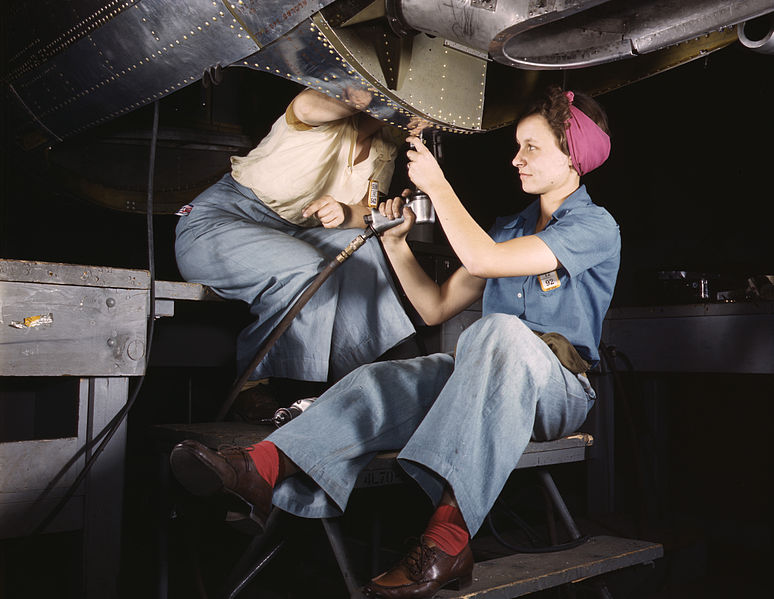
\includegraphics[width=10cm]{images/Women_working_at_Douglas_Aircraft.jpg}
    \caption{A "Rosie" performing manual riveting. wiki}
    \label{fig: rosieManualRiveter}
\end{figure}



The most popular and intuitive way is also the most traditional way of having a human operator hold a solid steel anvil acting as the base and another operator on the other side hammering the rivet using a simple ball pen hammer.This method requires a lot expertise, effort and time which makes it highly inefficient and impractical for big manufacturing industries.\\

Simple ball pen hammer way has been a standard in the past century but as we are living in the age of automation riveting has also advanced its methodologies. Instead of using man power to hammer we use special automated riveting machines.\\

The first method is to use a pneumatic hammer also commonly known as a riveting hammer in which the operator holds and directs the machine onto the rivet and then the machine hammers on the rivet with different intensities. Most of these hand held machines are pneumatically powered. These machines are ideal for applications where there is a need of agility to rivet at difficult angles and  limited space.\\

\begin{figure}[htp]
    \centering
    \includegraphics[width=10cm]{images/AutomatedRiveting.jpg}
    \caption{A fully automated riveting process. Boeing}
    \label{fig: rosieManualRiveter}
\end{figure}

Other method is to use a fully automated self sufficient riveting machine ie The fully automated machine automatically delivers and places the rivets in position and then squeezes the rivet in place fastening the materials together eliminating the need of a operator to organize the process. Such a process is highly consistent and accurate the making the whole procedure very efficient and cheap. Such a process is popular in aerospace and ship industry for fastening the skin of the product but the size and static working angle makes it difficult to deploy in tight spaces like while adjoining the fuselage pressure bulk head

\subsubsection{Industries involving riveting}

There are many methods of joining two materials together like soldering, welding, taping etc but riveting because of cost effective, straight forward installation and its ability to handle shear loads is still preferred as a favourable option industrial production. \\

Rivets are being used in building and construction industry specially when it is difficult to access the other side of the juncture, it is specifically used in building gutters and setting up the ceiling. It is also used in building big strong metal structures and towers like Sydney harbour bridges and Eiffel tower. ***** put a picture of each ******\\

Other rather more popular widely known industries are the aviation, aerospace and automotive industries. As there are many components in such machines it is important the parts are modular and can be repaired neat and easily but at the same time remain structurally strong and stable specially during motion which is rather difficult with other methods of fastening.\\

As there are many industries using rivets as industrial structural binder the methodologies and results of quality inspection with respect to rivets discussed in this thesis may not only be restricted to aircraft production and maintenance industry. 

\subsubsection{Industry quality standards}
    
    A flawless fastened rivet is an essential part of maintaining structural integrity of any machine and without doubt its of top most priority in ensuring the quintessential quality of safety critical machines like airplanes.
    \\
    \begin{figure}[htp]
    \centering
    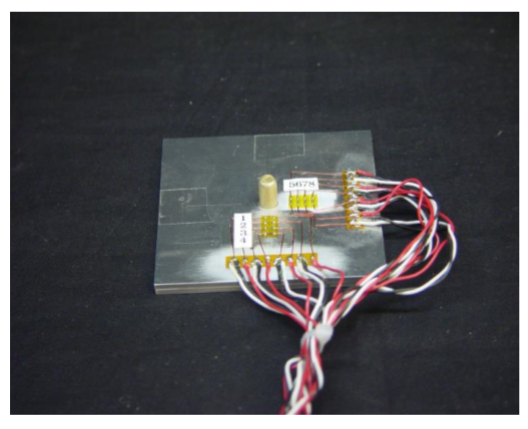
\includegraphics[width=10cm]{images/strainTest.PNG}
    \caption{ Micro-strain gauge arrangement on the inner sheet surface before riveting.  \cite{inbook}}
    \label{fig: strainGaugeTest}
\end{figure}

    There are various time consuming mechanical hand held measurement tools measuring the physical aspect of a rivet but again this technique is dependent on quality inspectors to go around millions of rivets which is a very time consuming and stress full process.
    \\
    
    In addition to the mechanical process of inspecting physical aspect of the rivets it is also essential to analyse the residual strain and interference experienced by the material being fastened.\cite{inbook} One could measure such fatigue by performing destructive and more suitable and efficient non destructive testing methods.\\
    
    

    
    The strain on the surface of the material can be measured by mounting micro strain gauges on interested positions.The total measured strain is the average of all the values measured in the covered area.\\
    
    The strain gauge method is good for measuring the strain on the surface of the material but for internal residual strain X ray and neutron diffraction  techniques is used which can penetrate deep into the sheets.The resultant strain value is the average of values measured each gauge volume.\\
    
    \begin{figure}[htp]
    \centering
    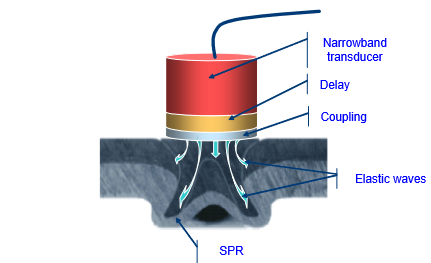
\includegraphics[width=10cm]{images/ultraSoundTest.PNG}
    \caption{ Operation Principle of transducer in the narrow band ultrasound resonance spectroscopy.  \cite{ultraSoundTest}}
    \label{fig: UltrasoundTest}
\end{figure}
    
    
    The narrow band ultrasound resonance spectroscopy 
    Another way of non destructive way to measure quality of the joint is ultrasonic  method which categorises the echo signal amplitudes as a function of interference or residual strain \cite{osti_191779} \\

    All such methods are convenient, reliable  and non destructive but have to be applied in conjunction to provide a comprehensive assessment which makes a general inspection resource and monetarily expensive. \\ 
    Also these tests are not convenient and scalable as special materials and infrastructure is required like putting on micro strain gauges around each rivet joint making the whole process more time consuming and cumbersome.
  
    Another essential methodology for quality check is visual inspection, in-fact more than 80\% of any inspection done on airplanes is manual visual examination. This approach is usually more faster an easily applicable at any time and place. 
    
    There are various aspects of a rivet that one has to consider while visually examining a rivet's quality.Typically there are 3 main defects that can be identified by visual inspection. \cite{FAA_visual_Inspection} 
    \begin{itemize}
    
    
        \begin{figure}[H]
        \centering
        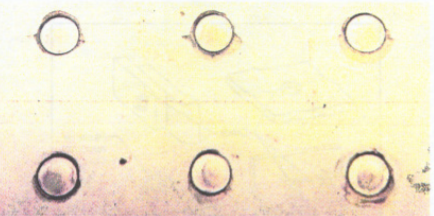
\includegraphics[scale=.8]{images/skincrack.PNG}
        \caption{Examples of skin cracking at fasteners. \cite{FAA_visual_Inspection} }
         \label{fig: rivet/skin crack}
        \end{figure}
    
        \item Cracks : Due to general wear and tear cracks originate on the rivet or on the surface which can over time and compromise the structural integrity. \\ 
        
        \begin{figure}[H]
        \centering
        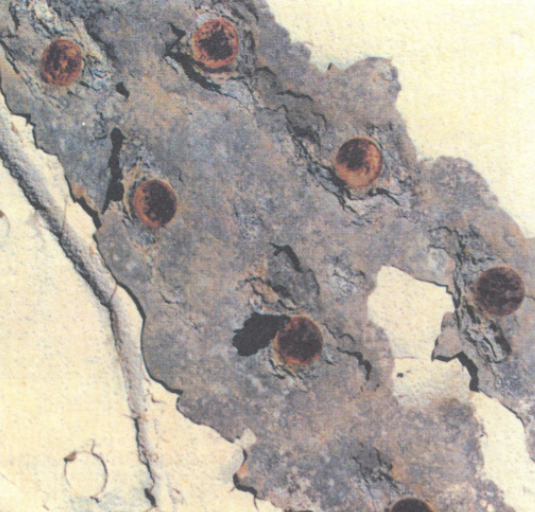
\includegraphics[scale=.5]{images/corrosion.PNG}
        \caption{Damage caused by corrosion. \cite{FAA_visual_Inspection} }
         \label{fig:corrosion damage}
        \end{figure}
        
        \item Corrosion : Places of juncture such as rivets are the most susceptible to corrosion and if not handled in time can infect the whole airframe structure.
        
        
        \begin{figure}[H]
        \centering
        \includegraphics[scale=.15]{images/DamagedRivet.jpg}
        \caption{Damage caused due to improper placement of rivetting hammer. }
         \label{fig:damagedRivet}
        \end{figure}
        
        
        
        \item Faulty installation: There is also a possibility faulty fastening during manufacturing which causes visible damage to the plates and rivets itself.
    \end{itemize}
    
    Also there are numerous other random defects that can occur by accidents, environmental factors etc which can be identified by visual inspection.
    
    

        
    
\quad \quad

\subsection{Human Robot Interaction}

Human-robot interaction is the multi-modular, interdisciplinary study of various fields like computer science, mechanical engineering, social sciences et all, to comprehend, design and evaluate of robotic systems improving the interaction dynamics between the human and robots and also reducing the mutual knowledge gap in an highly automated futuristic work environment. \\ \\
Human Robot interaction is considered a relatively novel field in the whole human machine interaction paradigm. There is a lot of work being done in labs to find new and feasible ways to interact with robots opening many more areas of application which were limited just humans or robots exclusively, like the use of robots for rescue in an urban disaster\cite{Murphy:2004:HIR:2220413.2220787} or in a more general day to day application like cleaning.\cite{cleaningRobot}.Human robot interaction also plays a vital role highly sensitive surgery procedures allowing robots to perform precise yet delicate actions.\cite{hriSurgery}\\
\\
Majority of interaction in big manufacturing robots is still limited to use of external computer systems to send and receive information from the robots.
The most important need in a industrial setup for a system to use human robot interaction is to maximise the workflow efficiency for both human and the machine and also providing human a relatively intuitive and safe environment to work in.\\

This thesis will be discussing on use of ubiquitous and modular ways using extended reality to interact with robots in a highly automated heavy machinery factory environment.

\subsubsection{Extended Reality (XR)}

Also acronymed as \textbf{XR} is a broader term relating to the technologies providing humans an alternate extended reality intertwined which actual reality adding new possible working paradigms to explore and utilise,in all improving on true potential of human capabilities.
Extended reality concept includes Augmented Reality (AR), Virtual Reality (VR) Mixed Reality (MR). To understand the relationship between all, Reality-Virtuality continuum is shown in figure . This continuum shows the transition between different realities and how are they arranged. \cite{reality-VirualContinuum}\\


\begin{figure}[htp]
    \centering
    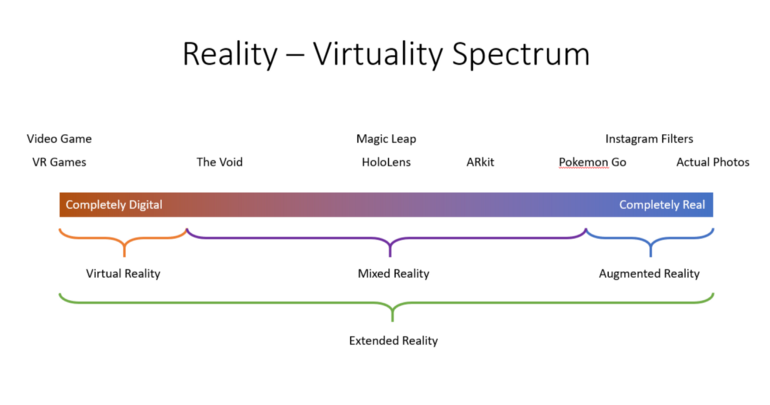
\includegraphics[width=10cm]{images/Virtual-RealityContinuum.png}
    \caption{Reality - Virtuality Continuum}
    
    \author{Jack Liu}
    \label{fig: V-RContinuum}
\end{figure}


\subsubsection{Virtual Reality (VR)}

\begin{figure}[htp]
    \centering
    \includegraphics[width=8cm]{images/VRExampleImage.jpg}
    \caption{Virtual Reality }
    
    \author{J. M. Eddins Jr/US Air Force}
    \label{fig: vRExample}
\end{figure}

Is an ability to experience a simulation or an alternate reality totally different from the real 3D space and time. This technology allows the human to immerse his/herself to different reality from his/her current reality with use of devices like VR glasses, headphones, actuators providing haptic feedback feeding alternate virtual environment information.\\



Such technology is popular among the entertainment industry with a games providing users with a novel and a totally immersive experience of playing games but at the same time it has also being used in more serious capacity like maintenance industries using it for performing remote quality inspection or control of robots, placed at tough environments like oil rigs, windmills etc. or used by scientist to explore and analyse inhabitable or extreme environments like space or deep sea explorations \cite{spaceAR} 

\subsubsection{Augmented Reality (AR)}

Augmented Reality
The literal translation of the word Augmented Reality means expanding(augmenting) the present reality. It is the technology which blends the real and virtual information with each other. It can be the real world overlaid onto a virtual application like the famous game "pokeman go" or virtual information supper imposed onto the real world using projectors or special AR glasses like Google glass, Holo-lens


\begin{figure}
%\hfill
\subfigure{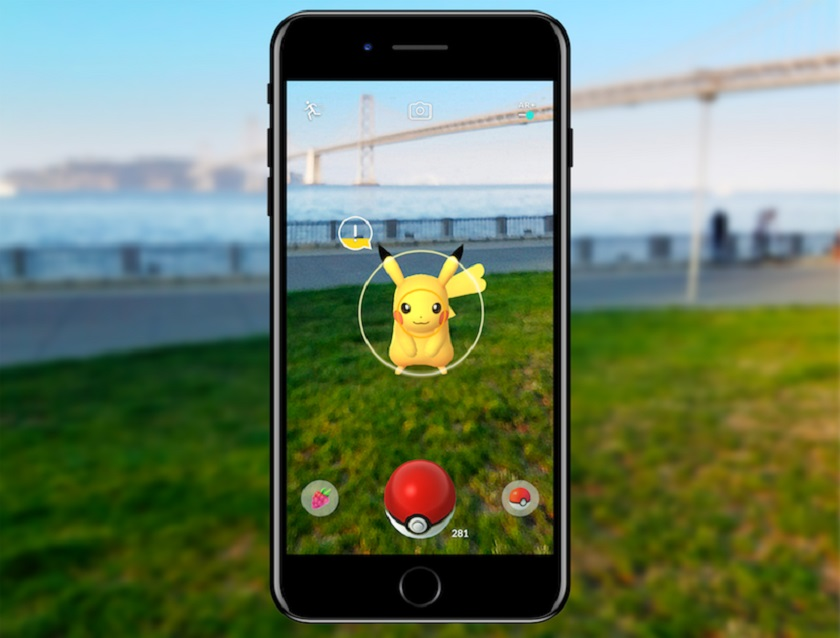
\includegraphics[width=5cm]{images/PokemonGo.jpg}
\author{[Niantic]}
}
%\hfill
\subfigure{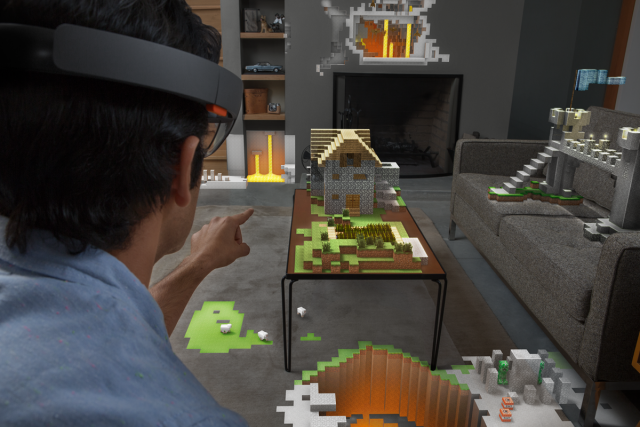
\includegraphics[width=5cm]{images/hololensView.png}\author{Microsoft}}
%\hfill
\caption{Examples of AR Application}

\label{fig: aRExample}
\end{figure}


\subsubsection{Devices}
    current alternatives to hololens,lenevo android , magic leap, wave 


\subsection{Classification Methodology}

Over the last decade, Artificial intelligence has gained much momentum and undoubtedly evolved from mere theoretical mathematical algorithms into a more open functional working capacity. AI backed systems are not only popular in the field of computer science but are also becoming an essential part of different fields across human civilisation development, from self driving cars to back end data analysis to fully automated smart factory floors and so on.\\

In the field of quality assurance, AI is extensively used especially in analysing data from various sensors of a machine. The classification model used in this thesis is powered by a series of Artificial Intelligence based classification algorithms.This Section gives a brief introduction to the Artificial Intelligence paradigm and how it can be used for classification. \\

\begin{figure}[htp]
    \centering
    \includegraphics[width=12cm]{images/artificialParadigm.PNG}
    \caption{Artificial Intelligence Paradigm.}
    \label{fig: Artifical Paradigm}
\end{figure}



\subsubsection{Artificial Intelligence}Is the design and implementation of a system which has the capability to perceive the provided environment and compute decisions which shall maximise the probability to achieve the predefined goal.
\\

\subsubsection{Machine Learning}Machine learning is a branch of artificial intelligence which includes special algorithms and statistical models that a computer can use to solve specific problems without any explicit instructions.
\\

\subsubsection{Un-Supervised Learning}A way of Machine learning technique which tries to find a relationship among the input data without being it labelled or categorised. In contrast to Supervised learning, during the training phase unsupervised learning considers only input space \(\mathbb{X}\) without any knowledge of out put \(\mathbb{Y}\). It recognises patterns, correlation based on input data's statistical properties. \\
The most commonly used unsupervised method is clustering analysis, They are mainly used to identify novel hidden patterns in the data or to identify anomalies where limited un-labelled data is available.

\subsubsection {Supervised Learning} A machine learning methodology in which the machine is able to learn by providing feedback to itself.The main goal of such a learning algorithm is to predict the outcome based on the relationship between the input variables. This relationship between the input variables is learnt during the training phase when each set of input variables results to the an output which then compared with labeled output provides a feedback on input variable's relationship.\newline\\
In more technical terms, let the input Vector space donated by \(\mathbb{X}\) and output space by \(\mathbb{Y}\). The input space has \textbf{n} samples and each sample having \textbf{k} features. Each sample X$_{i}$ = (x$_{1}$,x$_{2}$,$_{3}$, ... x$_{k}$) is mapped with a pre defined labelled output Y$_{i}$. 
With given (X$_{1}$, Y$_{1}$),(X$_{2}$, Y$_{2}$) ... (X$_{n}$, Y$_{n}$) the relationship should between should approximate to a function f(X$_{i}$)\newline\\
\centerline{Y$_{i}$ \sim f(X$_{i}$)}\newline

During the training phase the algorithm tries to learn the relationship between Y$_{i}$ and X$_{i}$ by minimising the difference be between f(X$_{i}$) and Y$_{i}$
\\

There are many algorithms categorised under supervised learning used for regression and classification namely linear and logistic regression, decision trees, Support vector machines, neural networks and so on.\\

Considering the characteristics of available data for this thesis custom designed and trained Neural networks were used for classification \\

\begin{figure}[htp]
    \centering
    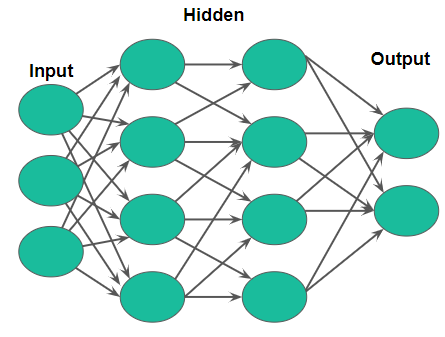
\includegraphics[width=10cm]{images/neuralNetwork.PNG}
    \caption{A typical Neural Network model.}
    \label{fig: Neural Network}
\end{figure}

\textbf{Neural Networks} : Neural Network is a highly specialised kind of supervised machine learning technique where the synthetic neural networks are inspired by biological neural networks.Such networks are organised in layers with each layer composed of multiple nodes/ neurons interconnected to each other and every such node represents the weight of that connection. With every pass forward and backward pass through the network during training phase these weights get updated minimising the distance between Y$_{i}$ and f(X$_{i}$)


\section{Problem statement}

On an average there are around 1.5 to 3 million rivets on a single commercial jetliner and it is of most importance to inspect each of these both at the time of production and maintenance.\\

As discussed in the previous "current industry quality section" There are already many techniques in place to perform quality inspection but this thesis identifies 2 areas were there could be improvements making the whole procedure of quality checks faster, effective and efficient.

\subsection{Lack of Real time intelligent Autonomous Quality Check }

The two most important aspects defining the quality of a rivet is the shape of affixed rivet and its structural and physical integrity.\\
In an typical visual quality inspection the following properties of a rivet should be inspected.

\begin{figure}[htp]
    \centering
    \includegraphics[width=10cm]{images/visualInspectionDeformaties.PNG}
    \caption{Rivet visual deformities. [AIRBUS, “Installation of Solid Aluminum Rivets”, Process Specification, 80-T-34-5814, Augsburg, 2008]}
    \label{fig:Visual inspecton deformaties}
\end{figure}

    \begin{itemize}
        \item Shape
        \item Diameter
        \item Width
        \item Angle to the base
        \item Any other physical deformity on or around the rivet.
    \end{itemize}



There are various time consuming and monetarily expensive quality inspection methods using mechanical hand held measurement tools assessing the physical aspect of a rivet but again these techniques are dependent on quality inspectors to go around inspecting millions of rivets which is a very time consuming, repetitive, tiring , mind numbing task leading to mental exhaustion which could lead flawed judgement.

\quad \quad \subsection{Absence of ubiquitous Operator robot Interaction}

At present the operator during production or maintenance is still reliant on cumbersome bulky computer systems to manage the tasks around and still have to rely on primitive screen or keyboard based interaction with the system resulting in following problems.

 \begin{itemize}

        \item No non intrusive way to interact with the robot system
        \item No way to receive information about system state in real-time
        \item Due to non intuitive way to control the robot special training is required to control the system.
        \item Special dedicated resource required to control the robot
        
    \end{itemize}



\section{Solution}

As mentioned in the previous sections it is of paramount importance to assure the quality of life liable machine like airplanes. To asses the mechanical structural quality of a rivet of an airplane one has to very precisely and diligently consider many visually evident and other non visual aspects of it.\\\\
In  the  field  of  quality  assurance,  AI  is  extensively  used especially in analysing data from various sensors of a machine.We provide two ways to inspect the quality of a aircraft rivet which could be deployed both at the time of aircraft production as well as during maintenance.\\\\
The solution is divided into two  modes,  an  online  mode  which  can be  used  to  asses  the quality  of  the  rivet  at  the  time  of  aircraft  production  as  well as maintenance and an offline mode which can be used during remote maintenance checks by airlines
    

\section{Concept Development}

The solution is organised such that it can provide a highly unique software and physical modular structure which collects and processes the data from various sensors and provides a final result.\\

The final solution aims to replace the human aspect of quality inspection by an intelligent automated process which determines the quality by classification based on images and physical parameters such as the height, diameter and force experienced while riveting in real time. The resulting quality information is then communicated to the operator via mixed reality glasses such as the Hololens. This allows for a more convenient way to manage maintenance work.\\\\
The development of the whole project can be divided into 5 sub tasks:

\begin{enumerate}
\item Setting up the Experiment
\item Data description and collection
\item Classification of rivet quality 
\item Training the neural network models
\item Deployment and final visualization of the results

\end{enumerate}




\subsection{Setting up the Experiment}


\begin{figure}[H]
        \centering
        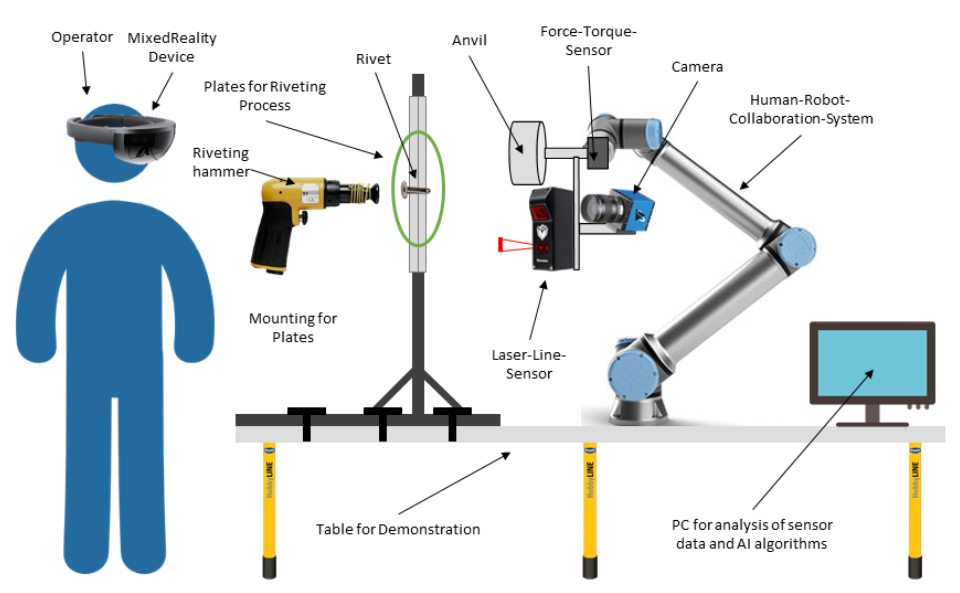
\includegraphics[scale=.5]{images/DemonstratorSetup.PNG}
        \caption{Experiment set up }
         \label{fig:ExperimentSetUp}
        \end{figure}

To confirm the feasibility of the solution a Universal Robot 10 (UR10) was used which scans along the fuselage  to perform quality check and passes the final information to the operator.The Robot is installed with a modular mounting onto which one could easily add or remove sensors as per requirement need.



\begin{figure}[H]
        \centering
        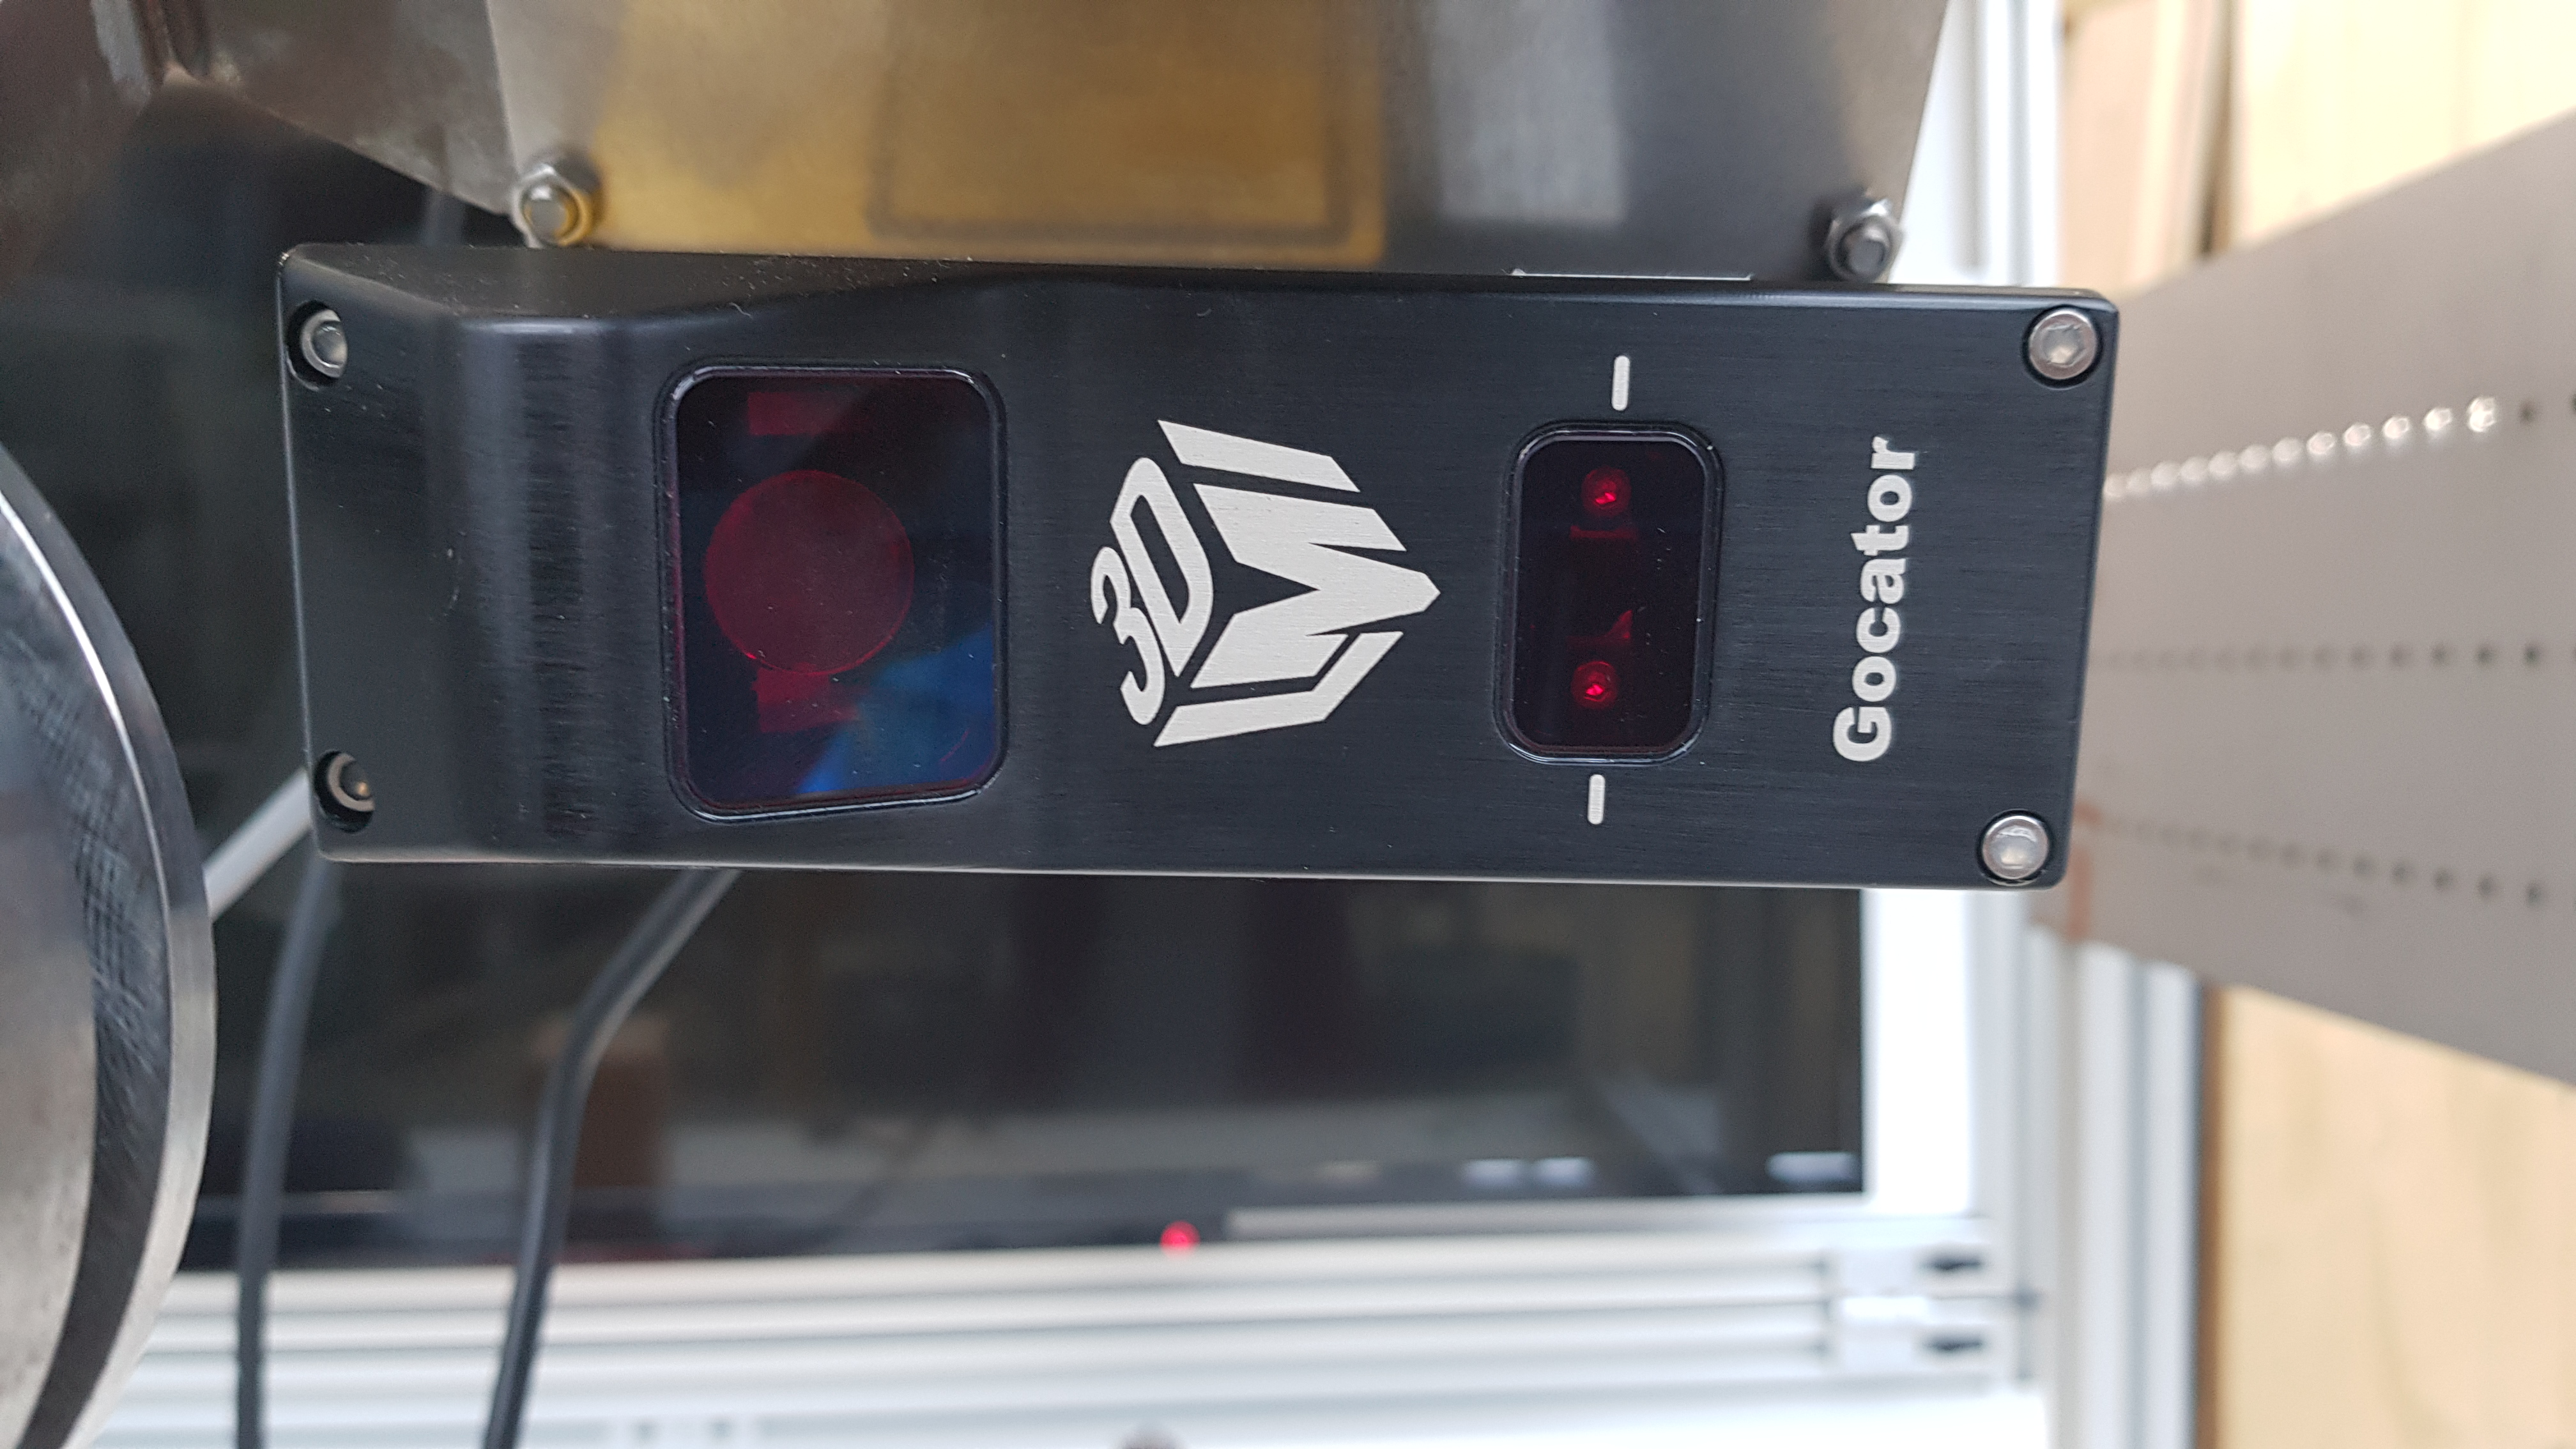
\includegraphics[scale=.07]{images/LMIsensor.jpg}
        \caption{LMI laser line 3D depth sensor.}
         \label{fig:LMIsensor}
        \end{figure}

For the concerned scenario of checking rivet quality , The quality check sensor module has a LMI 3D laser line sensor installed which scans through the surface rendering the exact shape of the rivet\\


\begin{figure}[H]
        \centering
        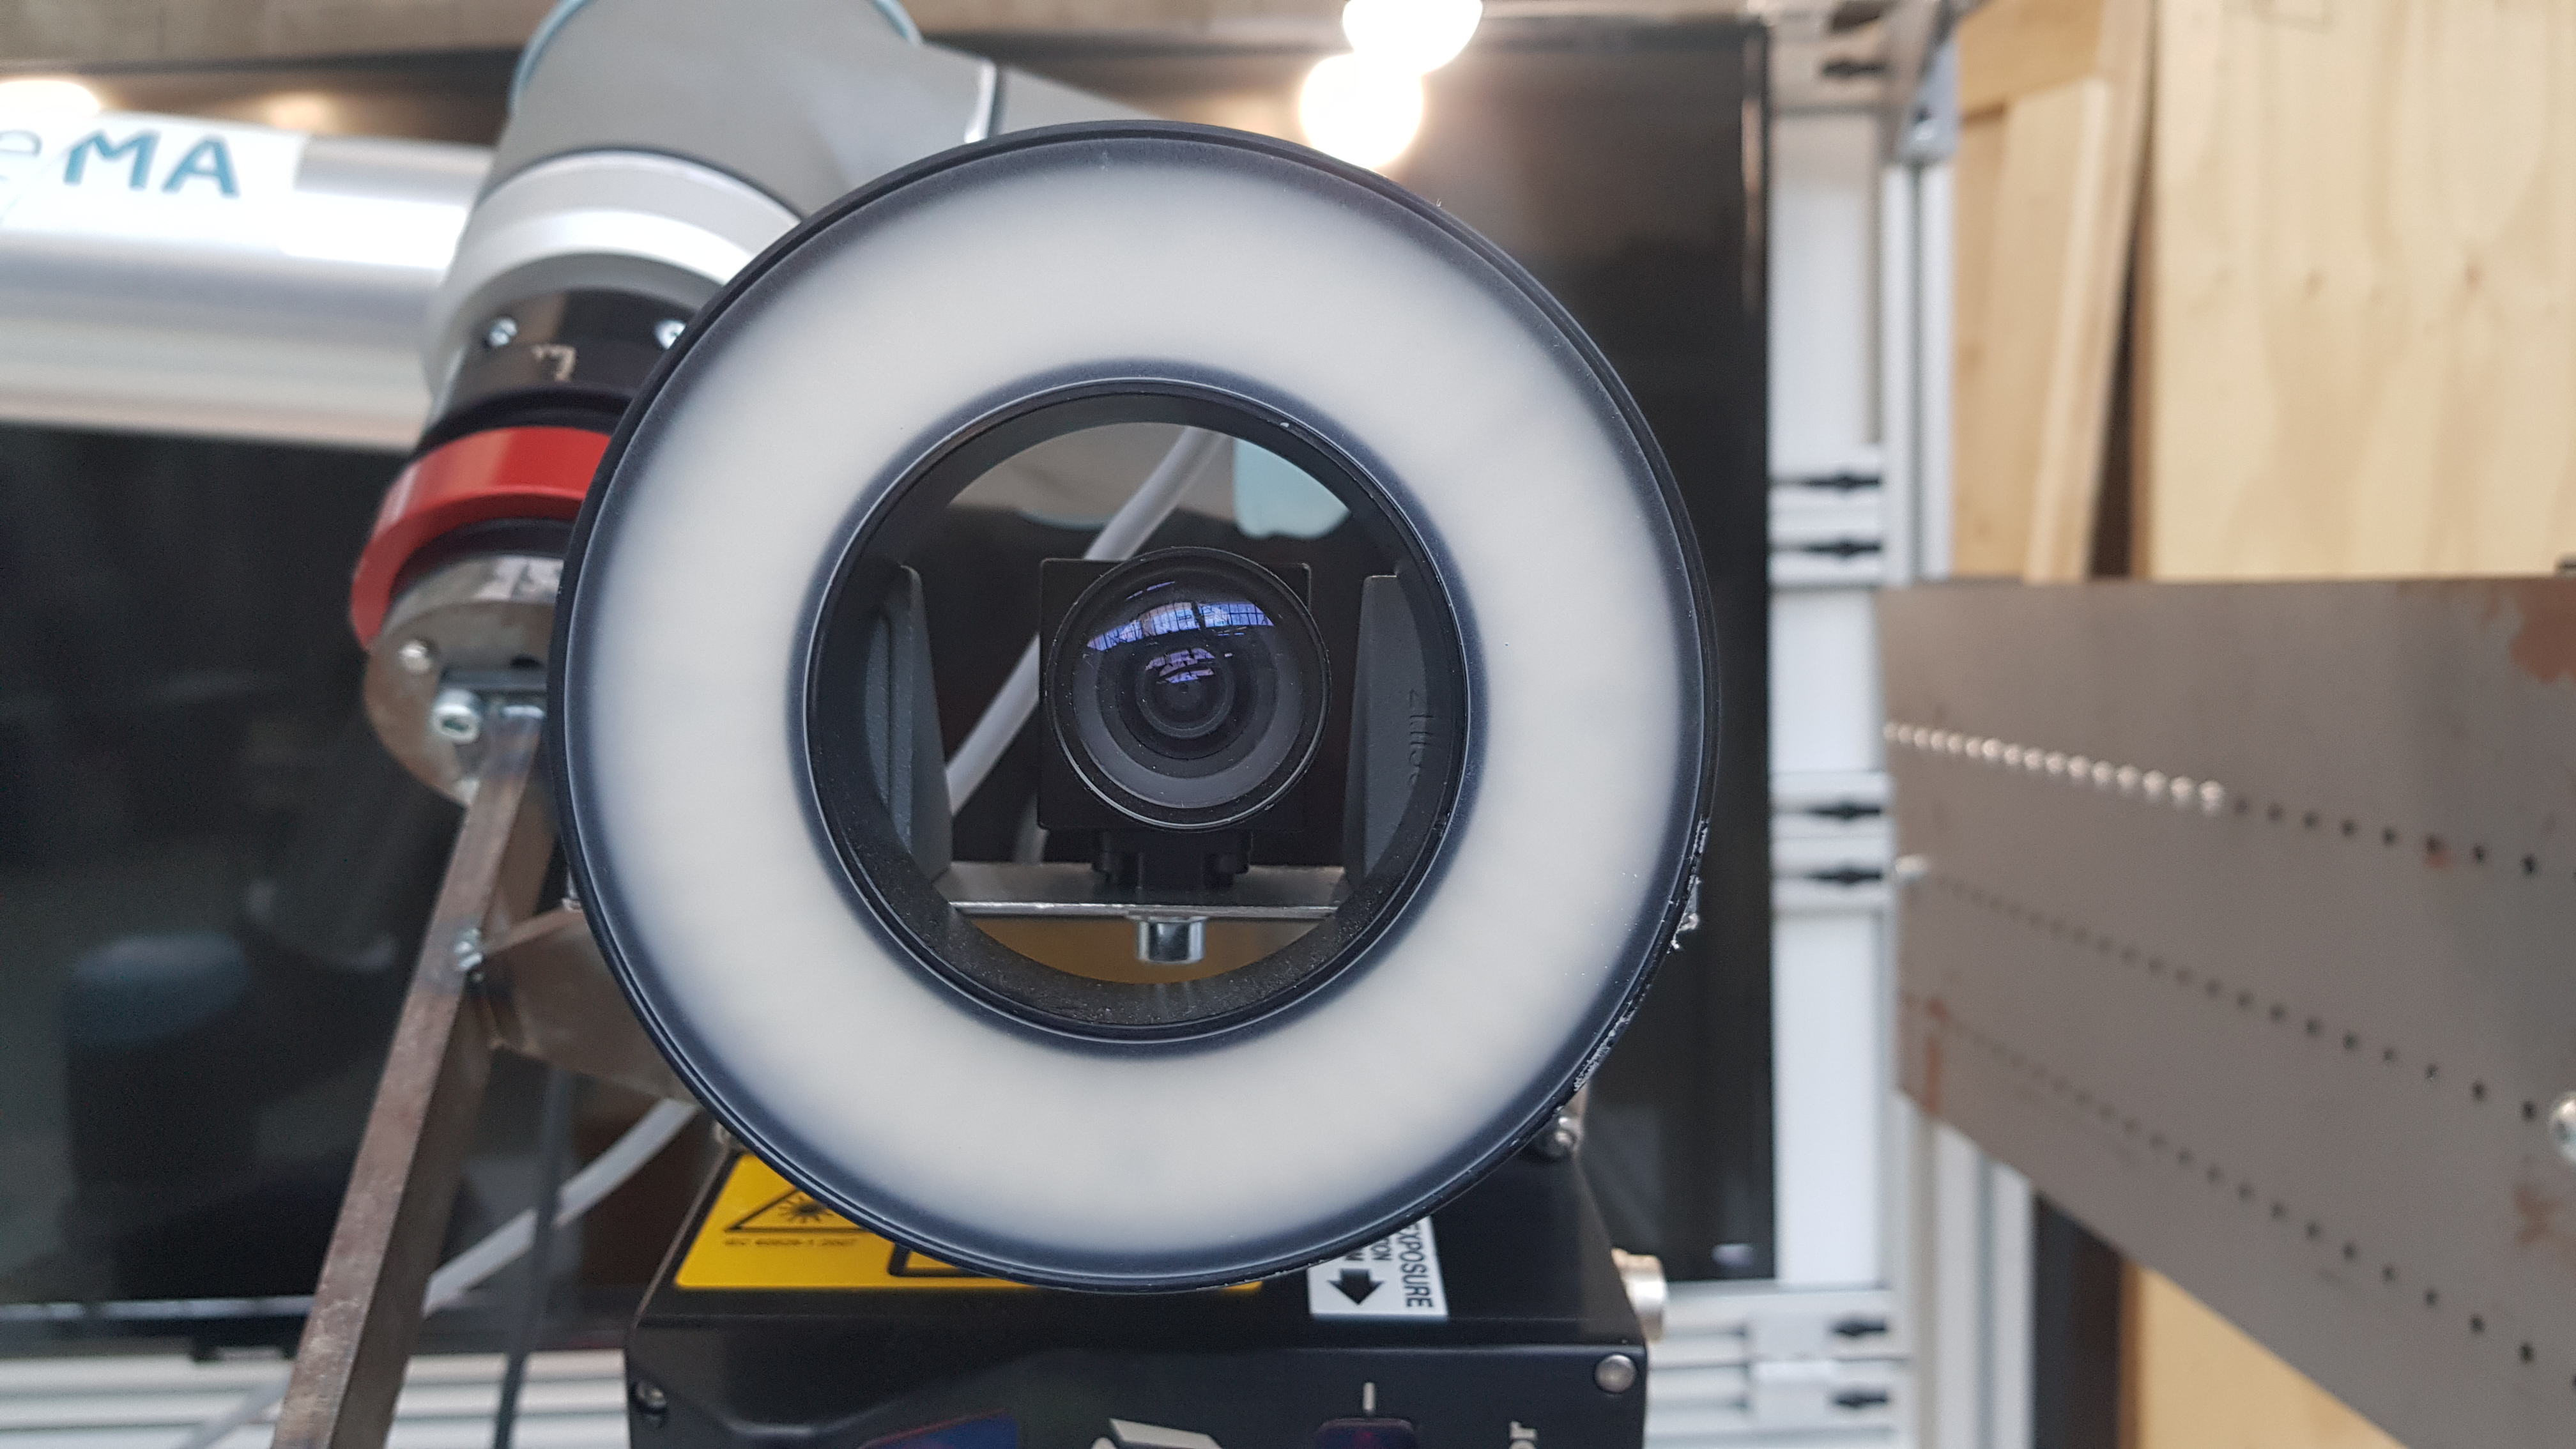
\includegraphics[scale=.07]{images/CameraSetup.jpg}
        \caption{Industrial grade RGB camera. }
         \label{fig:cameraSetup}
        \end{figure}
        
In addition to the laser line sensor there is mounted an industrial grade RGB camera along with a light ring providing consistent ambient lighting, taking pictures of the surface. Replacing the need of Visual inspection.\\


\begin{figure}[H]
        \centering
        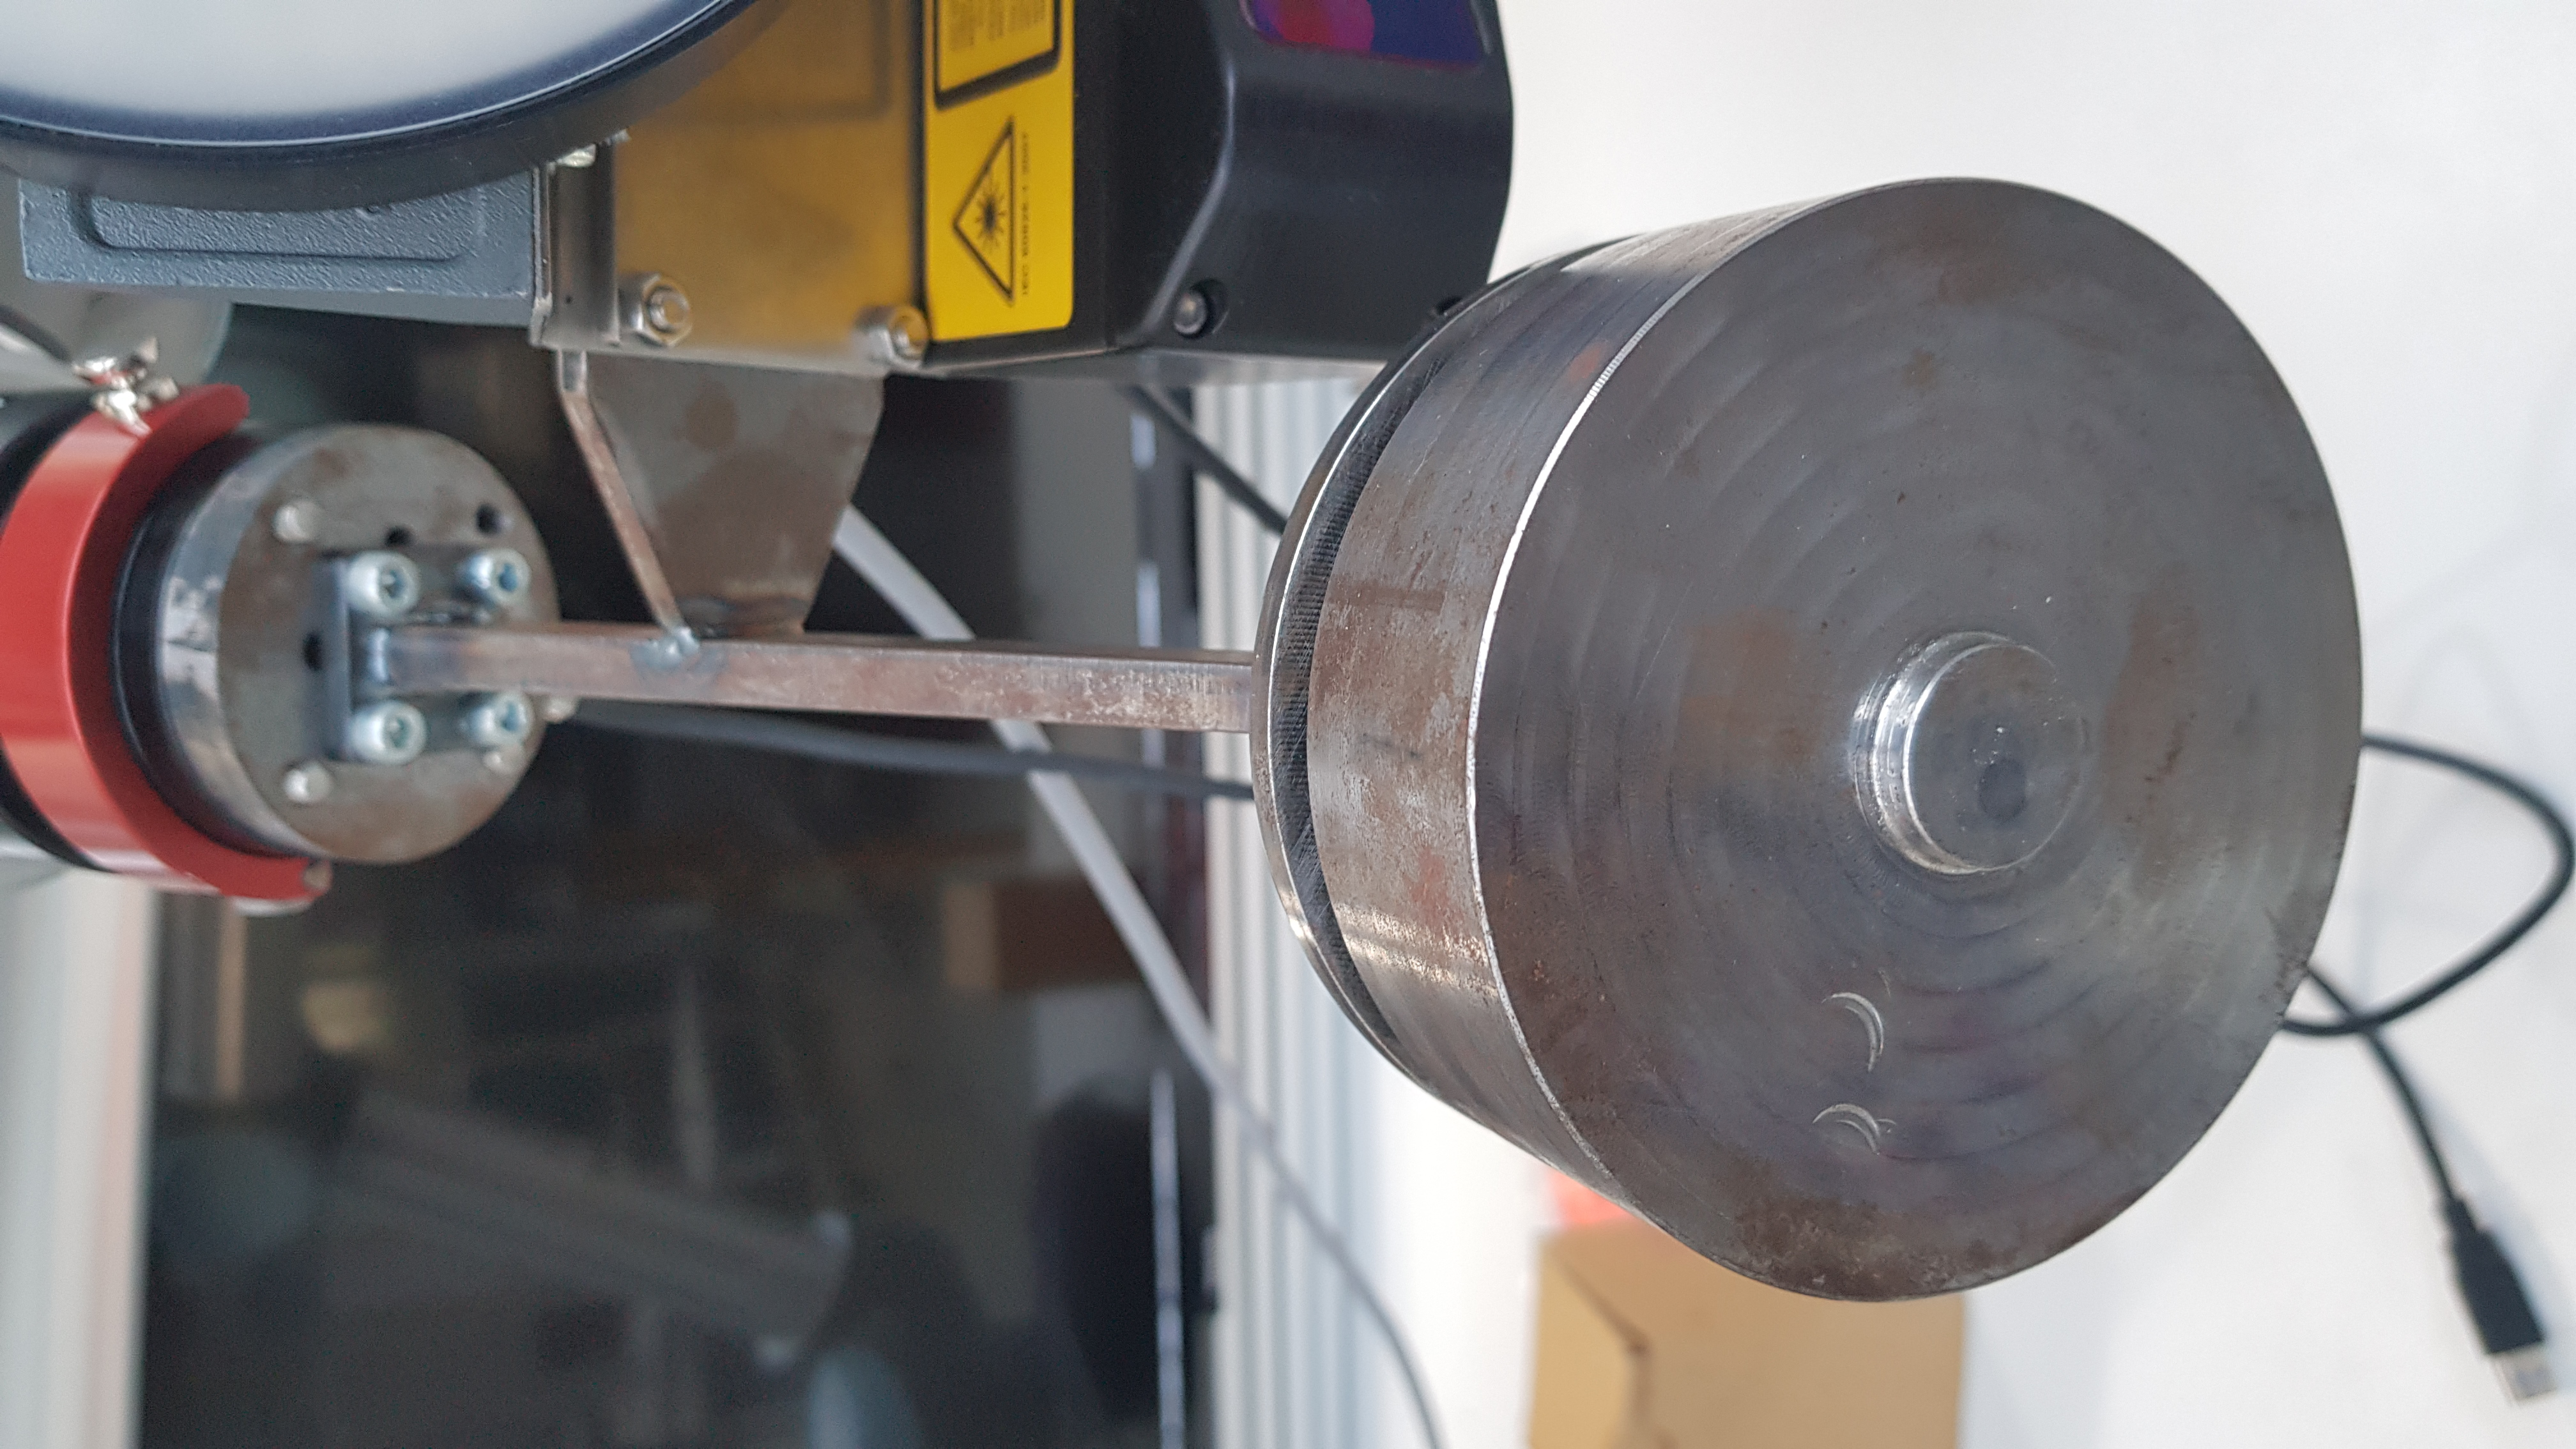
\includegraphics[scale=.07]{images/Ftsensor.jpg}
        \caption{Force Torque sensor. }
         \label{fig Sensor}
        \end{figure}

To support quality check at the time of production itself the also consist of a Force Torque Sensor, which measure the force experienced by the anvil while fastening of the rivet.

\begin{figure}[H]
        \centering
        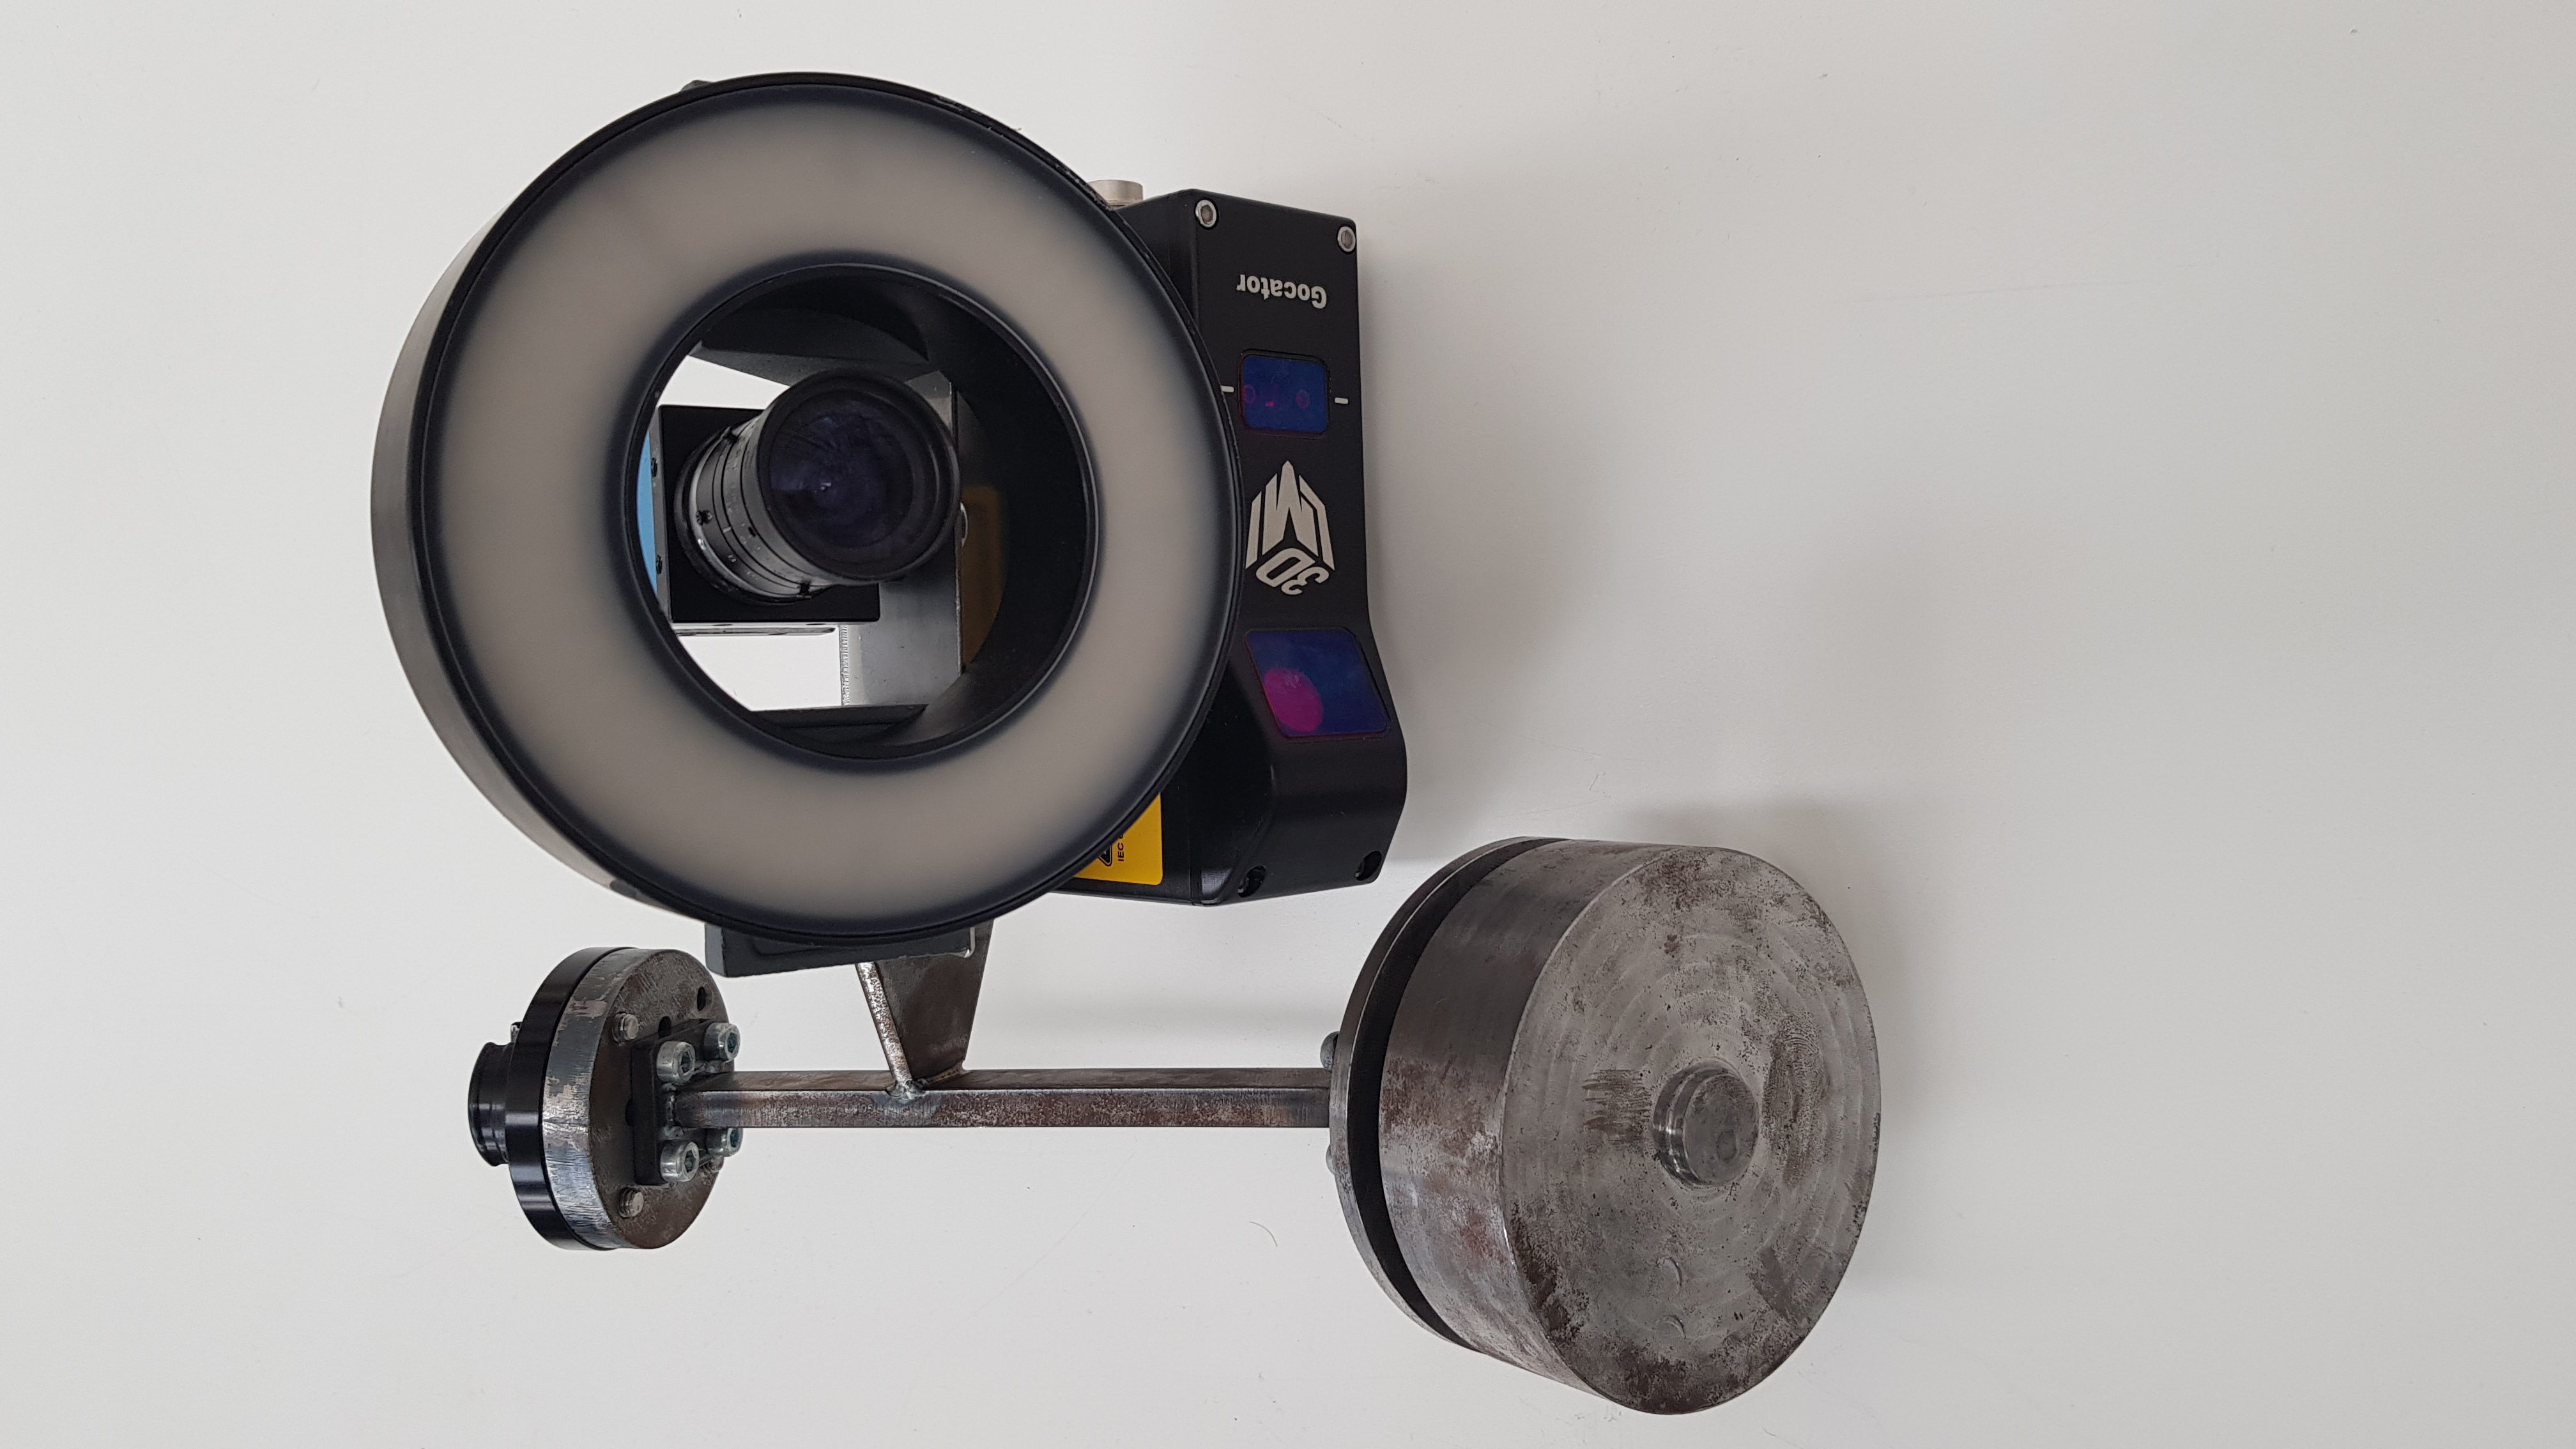
\includegraphics[scale=.07]{images/completeSetup.jpg}
        \caption{Modular installation mounting various sensors. }
         \label{fig:ModularSensorMounting}
        \end{figure}


\subsection{Data description and collection}

\subsubsection{Data description}\\
From all the above mentioned sensors a wide variety of data was collected which interm was pre-processed and used for training the classification model.
As mentioned earlier solid round head  rivets which are used for joining the pressure  bulkhead of an airplane with the fuselage were considered.These are one of the most common and reliable kinds rivets used across all industries. \\

The camera setup includes an industrial grade camera along with an ambient light ring. This setup is mounted on to the robot which allows the camera to move around and place itself right in front of the concerned rivet putting it in focus. 
It provides with 640 by 480 resolution coloured image having consistent ambient light exposure allowing the tool to operate in all kinds of lighting conditions.\\

\begin{figure}[H]
        \centering
        \includegraphics[scale=.4]{images/cameraOutputImage.png}
        \caption{Image of rivet with consistent ambient light exposure. }
         \label{fig:cameraOutputImage}
        \end{figure}


The laser line sensor is capable of xxxx depth readings in a minute, It measures its distance to the material while it moves over the rivet providing a 3D point cloud of the surface, which infact is used to deduce important information like height and width of the rivet.\\
The height is measured by calculating the difference between depth of the highest point in the frame and the depth of the plate itself. The sensor is also programmed to deduce the diameter of the rivet in X and Y directions. Using all the above information the shape of the rivet is assessed including the its angle to the base.\\\\


\begin{figure}[H]
        \centering
        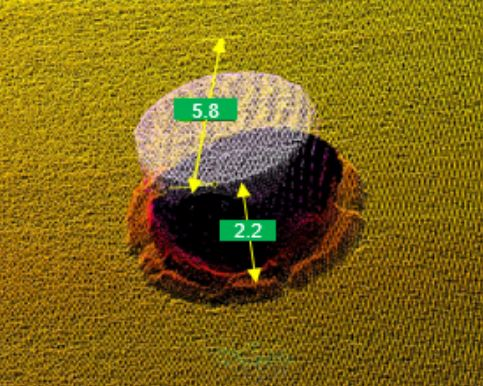
\includegraphics[scale=.8]{images/3dPointcloud.JPG}
        \caption{3D point cloud of a rivet by laser line sensor. }
         \label{fig:}
        \end{figure}


As shown in figure \ref{fig:forceExperienced} shows the force torque sensor records the force experienced by the anvil in all 3 X,Y and Z dimensions during the time of fastening of the rivet itself.

\begin{figure}[H]
        \centering
        \includegraphics[scale=.8]{images/force.png}
        \caption{Force experienced by the anvil in all 3 dimensions.}
         \label{fig:forceExperienced}
        \end{figure}

\subsubsection{Data Collection}

Training a machine learning model requires a lot of data to provide reliable generalised results hence a simulation of real riveting process was set up.\\

\begin{figure}[H]
        \centering
        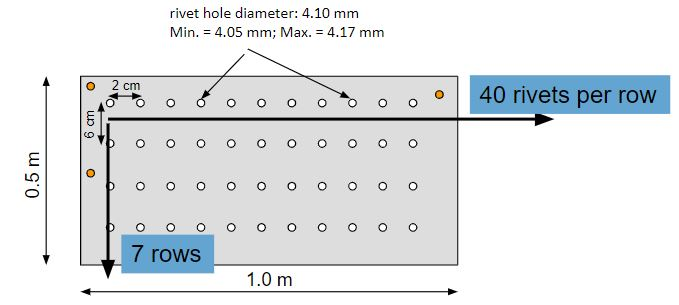
\includegraphics[scale=.8]{images/airplaneFuselageSimulation.JPG}
        \caption{Aircraft fuselage simulation setup}
         \label{fig:Aircraftfuselagesimulationsetup}
        \end{figure}

To imitate the fuselage two 2 mm plates with holes of diameter with 4 mm placed at least equivalent to 3 x rivet diameter (1.2 cm) distance apart from  each  other and 2 rivet diameter (8 mm) apart from the corner were used.Each plate had 7 rows of 40 rivet holes hence accommodating 280 rivets per plate.\\

In total 9 such plates were used to fasten 2545 rivets by experts collecting data from the laser line sensor, Ft sensor , images for each and every rivet. The riveting procedure was divided such that to create both good and bad rivets which is evenly represented in the collected data to train a balanced classification model.\\

\subsection{Data Pre-processing and Labeling.}

\subsubsection{Data Pre-processing}

Data pre-processing is the process of transforming raw data into usable sense full data for the learning algorithms to train on. It is the first and one of the most significant step of machine learning Process.\\

\begin{figure}[H]
    \centering
    \includegraphics[width=10cm]{images/MlProcess.PNG}
    \caption{Data pre processing in machine learning process}
    
    \author{David Chappel}
    \label{fig: machineLearningProcess}
\end{figure}

Generally the real world data is very noisy, incomplete and even incomprehensible to the machine hence it is essential to perform some processing to clean, extract the most important features and make it machine readable to pass it through machine learning training process to find relation and patterns among it. Data pre-processing includes the process of \cite{Kotsiantis06datapreprocessing}

\begin{itemize}
 
    \item Data Cleaning
    \item Data normalization
    \item Data transformation
    \item Data labeling
    \item Feature extraction and selection.
    \end{itemize}

\textbf{Image Data: }
For every rivet an coloured image was taken focusing onto the front/face of the rivet to identify any cracks or other physical deformities.Each Image had a 640 X 480 pixel resolution.Following pre-processing was performed on the image data\\

\begin{figure}[H]
    \centering
    \includegraphics[width=10cm]{images/ImagePreProcessing.PNG}
    \caption{Image Data Pre-Processing}
    \label{fig: ImageDataPreprocessing}
\end{figure}

 \begin{itemize}
     \item The data was collected such that the concerned rivet is always approximately in the middle of the frame and most quality defining features are on the rivet itself or the immediate area surrounding it, a 100 X 90 resolution image was cropped out from the center concentrating on the rivet which resulted in omitting all the unnecessary data.
     \item To reduce any sharp effect due light reflection, each image was passed through a Gaussian blur filter.
     
     \item In a Visual inspection of a rivet the important information is presence of any physical deformities hence color of the rivet is irrelevant. To remove this redundant information each image was converted into a gray scale image.  
     
     \item As the shape of the rivet and cracks are the most looked out features for classification an edge detection kernel was convoluted onto it highlighting the exact shape of the rivet and also if present any irregular deformities  
     
    \end{itemize}



\\\textbf{Force-Torque Sensor Data: }
    
FT sensor directly mounted on to the robot measures the force experienced by it during fasting of the rivet in all 3 X,Y and Z. the force data was collected over 500 timestamp data points for every rivet.



\begin{figure}[H]
    \centering
    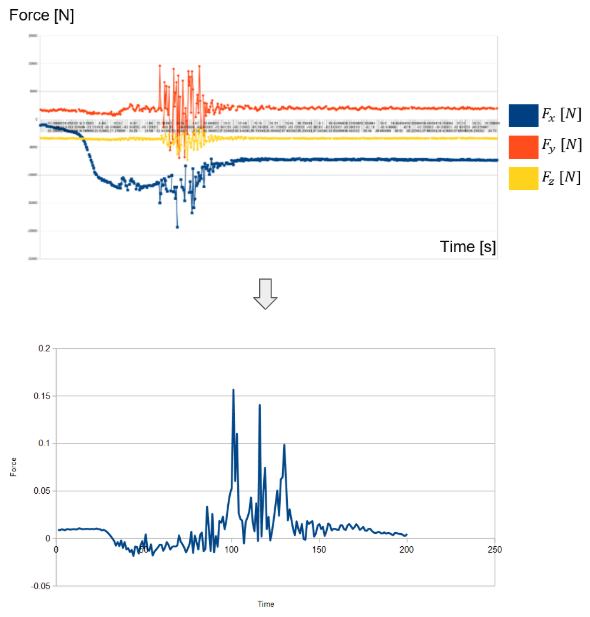
\includegraphics[width=10cm]{images/FTdataPreProcessing.PNG}
    \caption{Force Data Pre-Processing}
    \label{fig: FtDAtaPreProcessing}
\end{figure}

\begin{itemize}
    \item Depending on the position of the rivet and the robot’s posture each dimension poses important characteristics therefore and average of forces along all three axis is considered.
    \item As the riveting is done by a human hence the riveting timestamp across different rivets is not synchronised. To align the interest  points across all rivets the point with highest  force was identified and 100 points before and after the highest point were filtered in. These are the points with most features and represent the duration of actual contact between the hammer and the  rivet.
    \item The data was also rescaled between -1 to 1 to keep the data consistent among different rivets and represent the actual scale of riveting force features.
\end{itemize}

\subsubsection{Labelling}

Once the data was acquired from all 2545 rivets, It was labelled by an expert to facilitate  the training process. Each data point was categorized as a ‘good’ or ‘bad’ rivet on various parameters such as dimensions measured by the laser line sensors and the image of the rivet head.

\begin{figure}[H]
  \centering
  \subfloat{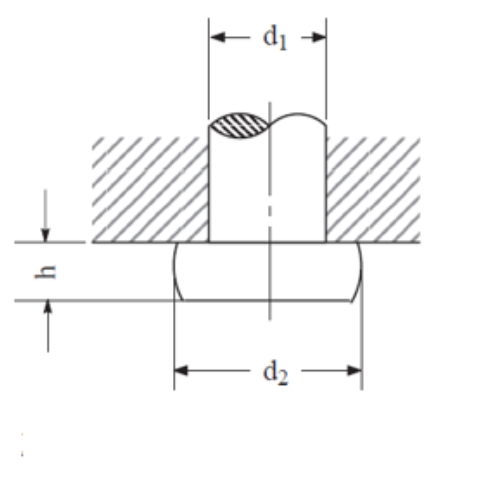
\includegraphics[width=.6\textwidth]{images/labelRivetDimension.PNG}}
  \hfill
  \subfloat{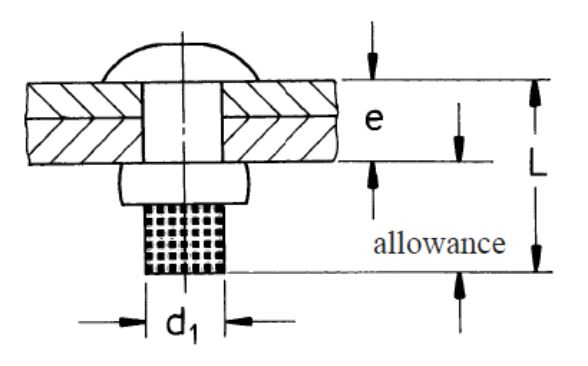
\includegraphics[width=.6\textwidth]{images/variablesDefiningRivetDimensions.JPG}}
  \caption{Variables defining rivet dimensions}
  \label{fig:RivetLabelVariable}
\end{figure}




Collected data was labelled based on the criteria defined by airbus specifications \cite{airbusRivetSpecification} and \cite{FAA_visual_Inspection}

\begin{itemize}
    \item  Each rivet's final dimensions (Figure\ref{fig:RivetLabelVariable}) were compared with the qualifying acceptable range.
\\ \[ d_1 \leq 4mm :  L = e + 1.5d_1 \]
With respect to the equation and our experiment specification, a good rivet's diameter lies in the range of 5.6mm to 7.5mm and its height in the range of 1.3mm to 2.6 mm as per airbus specification show in in figure\ref{fig:goodRivetRange}. Hence all rivets having physical dimensions outside the specified range were labelled as "bad" 

\item Rivet was also assessed based on the shape and any other visual features to the rivet head or the surrounding plate.A visual damage could be cracks or physical deformity due to improper posture of the riveting hammer while riveting or use faulty rivet die.Some cracks may also appear due stress experienced by the rivet over a period of time and lack of thorough maintenance.
\end{itemize}

In  accord  with  visual  inspection  1023  rivets  were  categorized ”bad” and 1522 rivets were labelled ”good” and as per the physical dimensions 964 are labelled ”bad” and 1437 as good

\begin{figure}[H]
    \centering
    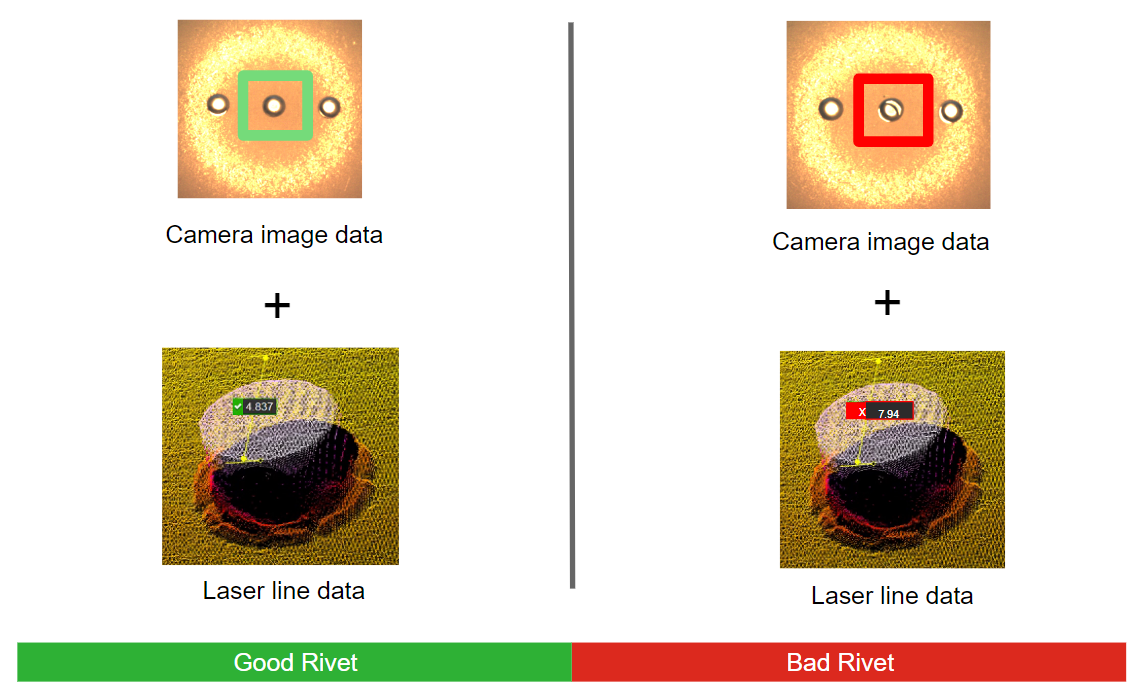
\includegraphics[width=11cm]{images/goodVsBadRivet.PNG}
    \caption{Good Vs Bad Rivet characteristics}
    \label{fig:goodVsBadRivet}
\end{figure}

\subsection{Classification of Rivet Quality}

The Whole classification model is based on the conjunction of quality results from 3 main sensor inputs.

\begin{itemize}
    \item Image of the rivet head
    \item Force Experienced during fastening
    \item Shape of the rivet deduced by Laser Line sensor
\end{itemize}


\subsubsection{Image Data Classification model}
Convolution neural networks \cite{Krizhevsky:2017:ICD:3098997.3065386} were used to classify the rivet into "Good" or "Bad" based on its image.

** image of training augmentation **\\

CNN requires considerable size of training data hence there was need to augment the data. Each rivet image was rotated horizontally resulting in a new augmented image data set of total 28150 training images. All images were also rescaled to 36 X 36 resolution for faster and less resource consuming training.

\begin{figure}[H]
    \centering
    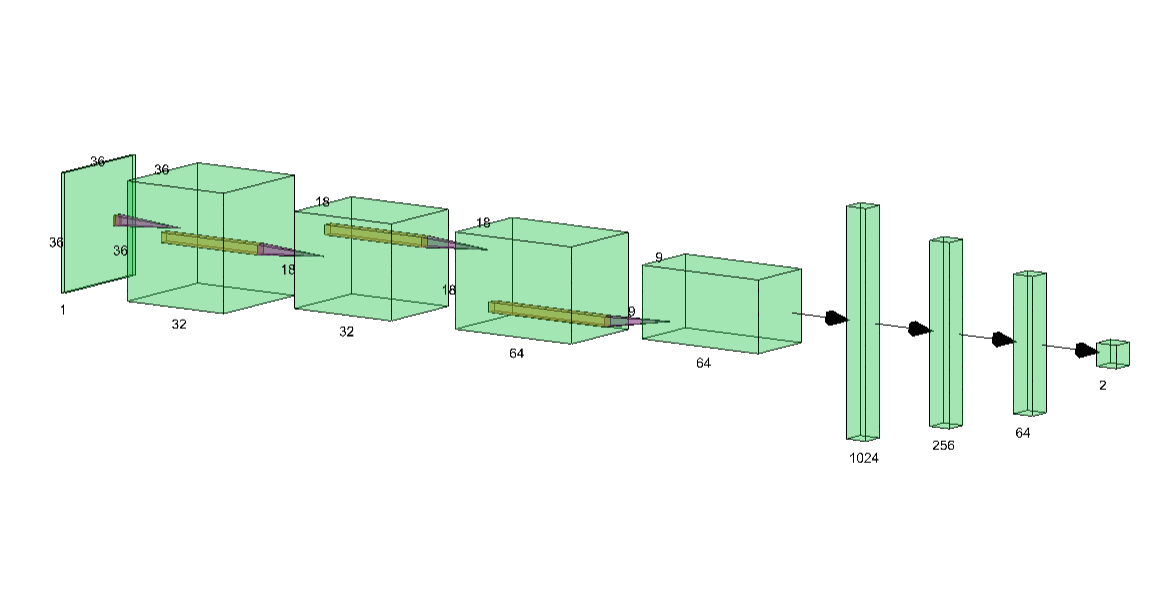
\includegraphics[width=12cm]{images/CNN.PNG}
    \caption{Convolution Neural Network Architecture}
    \label{fig:ConvolutionNeuralNetworkArchitecture}
\end{figure}

The Final CNN model has of 36 X 36 data point input passed to the 1st Convolution layer - max pooling layer combination with convolution layer having 32 filters and max-pooling having a pool size of 2 x 2, subsequently connecting it to the second Convolution layer with 64 filter and max pooling layer of 2 x 2 pool size. Out put from the previous layer is passed to a deep network having three layers all densely connected, organised into a 1024 X 256 X 64 X 2 neuron  architecture with each having a dropout rate of 25\% to help counter over fitting.

The model was cross validated using K-fold cross validation with K = 10. Each group was trained over 20 epochs with a batch size of 10. Average test accuracy of 98.2\% was observed over all 10 groups.

\subsubsection{Force torque Data Classification model}

The pre-processed Force torque sensor data was used to classify a rivet into a "Good" or "Bad" by training a Deep neural network.

The DNN model has an architecture having 200 neurons at the input layer representing the relevant timestamp points of each rivet's force data.This layer is densely connected to a deep network with 1st layer having 100 neurons and 2nd layer having 50 neurons each having Relu as their activation function with 20\% dropout rate. Final the output neuron is connected to the second layer having sigmoid activation function.

For training of Ft data DNN a conjugate of label data based on rivet dimensions and image data was taken giving only mere 300 good data and 300 random bad data points. Training and Test is divided into 70-30\%. The trained model gave a test accuracy of 85\% accuracy which given to the nature and limited amount of data is acceptable as per the industry standards and shows much promise in the methodology.

\subsubsection{Laser Line sensor Data Classification model}

Classification of a rivet using a Laser line sensor data was done using a much primitive rule based classification. If the dimensions of the rivet were under the certified range it was categorised as "Good" and if not in range it was classified as "Bad" as discussed in section 6.3.2 following category of rivet was used.

\begin{figure}[H]
    \centering
    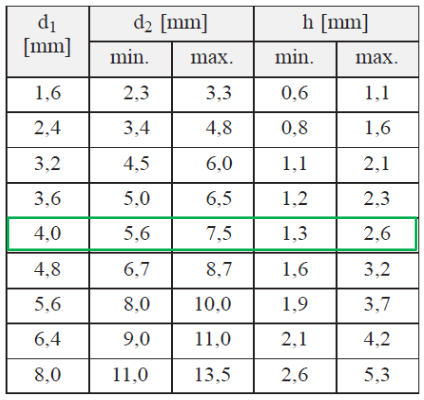
\includegraphics[width=6cm]{images/goodRivetRange.PNG}
    \caption{Good Rivet dimension range}
    \label{fig:goodRivetRange}
\end{figure}


\subsubsection{Over all Classification}

Final classification of a rivet considers the results from all three sensor classification models and then pass it through a custom designed logic gate. \\\\
For each sensor classification model depending on the confidence with which a model predicts the quality of the rivet the result could be divided into 3 categories 

\begin{itemize}
    \item "Good" : When the model predicts with more than 85\% confidence that the rivet quality is Good
    \item "Needs attention" :  When the model predicts with confidence between 50\% - 85\% that the rivet quality is Good or Bad
    \item "Bad" : When the model predicts with more than 85\% confidence that the rivet quality is Bad
\end{itemize}

The Final logic gate is defined such that if any of the sensors classification model predict that the rivet is "Bad" the final quality result is Bad, if any of the sensor's data model predict "Needs attention" and rest predict that the rivet is "good" then the rivet needs a second look from the quality inspector and if all sensor data models predict that the rivet is "Good" then the rivet is of Good quality.


\begin{figure}[H]
    \centering
    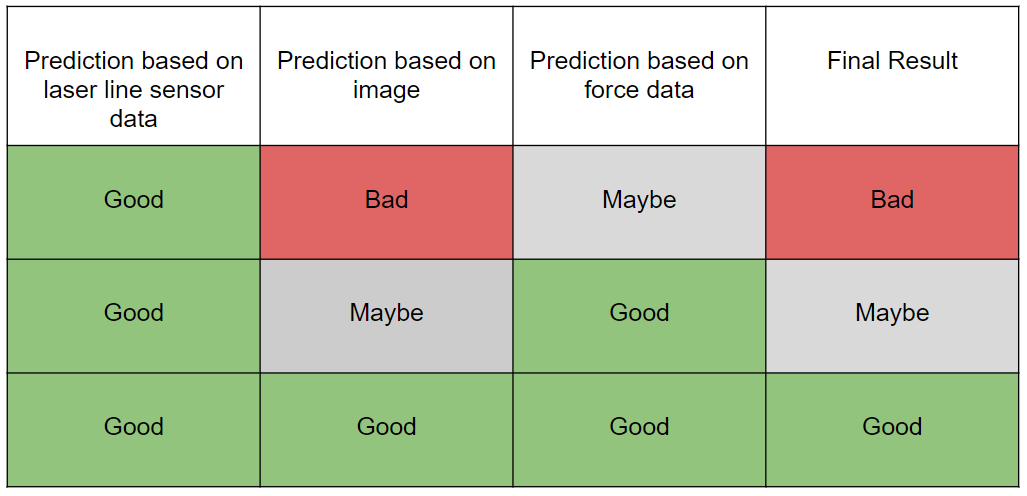
\includegraphics[width=12cm]{images/logicTable.PNG}
    \caption{Logic deciding final result}
    \label{fig:finalResultLogic}
\end{figure}


Process flow of the overall quality check procedure is divided into two modes supporting two different use cases.



\begin{figure}[H]
    \centering
    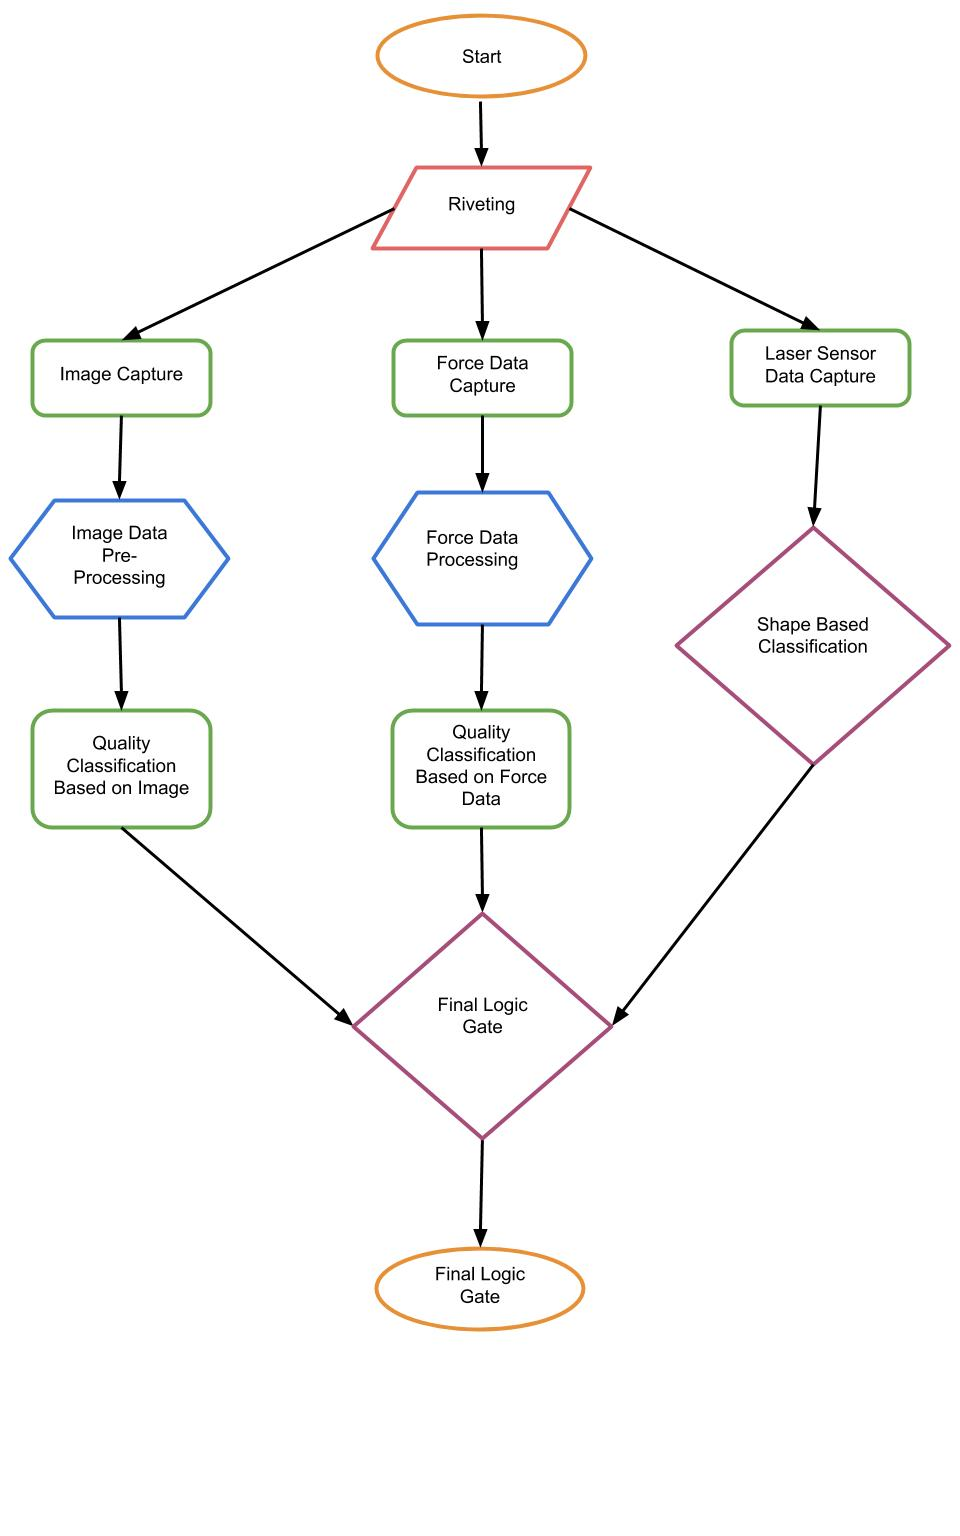
\includegraphics[width=10cm]{images/OnlineQualityMode.jpg}
    \caption{Online Quality Mode Process Flow}
    \label{fig:OnlineQualityModeProcessFlow}
\end{figure}

\textbf{Online Mode :} Mode of inspection which can be used to asses the quality of the rivet at the time of aircraft production as well as maintenance. In an online quality inspection the system is capable to evaluate the quality of the rivet at the time production itself. Data from force torque sensor and laser-line sensor and camera is used to classify the rivet into a "good" and "bad" quality category.

\begin{figure}[H]
    \centering
    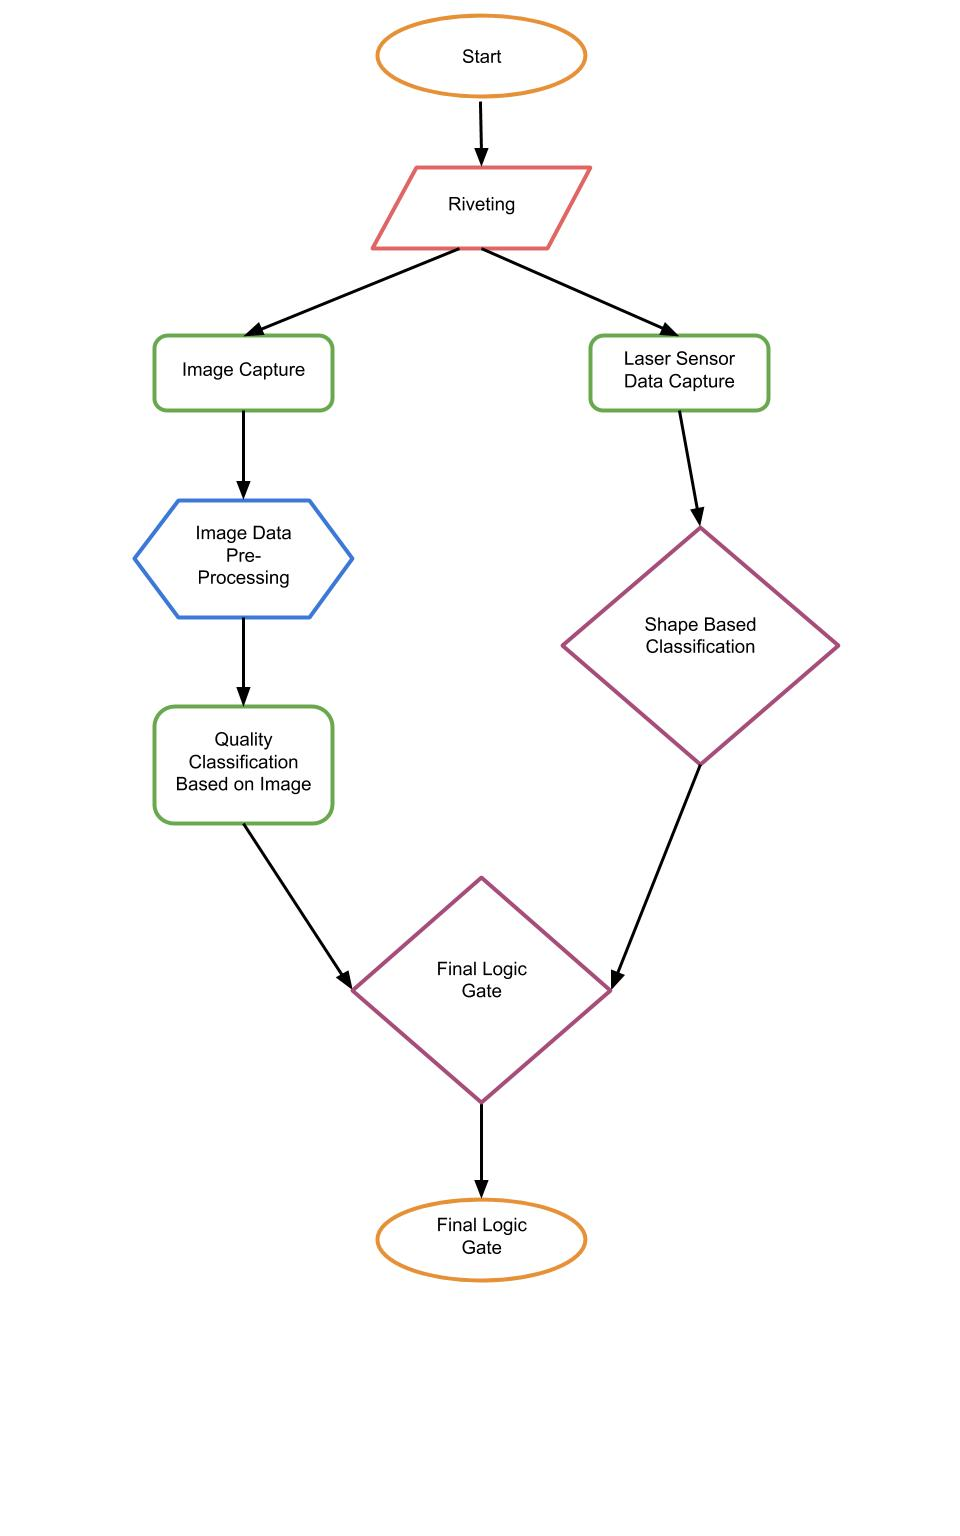
\includegraphics[width=10cm]{images/OfflineQualityMode.jpg}
    \caption{Offline Quality Mode Process Flow}
    \label{fig:OfflineQualityModeProcessFlow}
\end{figure}

\textbf{Offline Mode :} As an alternative to the online mode of quality inspection, offline mode provides a capability to asses the quality after the riveting procedure, particularly focused towards maintenance tasks.\\ 
In this mode the system considers the shape and image of the rivet and classify into "good" or "bad" particularly eliminating the need of manual visual inspection by the quality inspector.


\subsubsection{Result Visualisation}

In a smart factory setup a fluid flow of workflow is always desired for maximum efficiency and specially when there is a machine and human working together in  same space.\\

To provide a comprehensive solution this thesis complements the autonomous quality inspection with a  novel yet highly intuitive way to interact and visualise the final result using Augmented Reality. It provides a duplex technique of communication in which not only the operator is able to send commands to the robot but also the robot could communicate its current status and updates to the user in a more ubiquitous manner.\\

A hololens application was developed which allows the operator to conduct general inspection in collaboration with the robot in a totally hands free ubiquitous natural manner.\\

The application supports 2 floating menu's in the form of holographs which can be accessed at any time by the operator using gestures. These menu's allow the operator to control the robot or command the robot to reinspect if such a need arises.\\ 

*** image of the closed and open menus ***

All the communications between the robot and the hololens is handled by a custom build ROS bridge library powered by web-sockets connections.\\

Hololens application includes a complete virtual smart factory environment in the form of holographs
superimposing the real machines allowing the operator to have clear view of the mechanics even hidden behind the fuselage. *** image of unity scene *** 


By scanning a unique QR code the application is able to locate the exact location and orientation of the physical environment and hence allowing it to anchor and place the virtual holographs relative to the respective real physical counterparts.\\

** image of the holograph highlighting bad rivet ***

Once the system is classified the rivet as "Good" or "Bad" Using similar methodology as mentioned above it is able to locate the exact position of the problematic rivet and highlights it by placing a red holographic marker around it. This allows the operator to easily identify and locate the "Bad" rivet among millions of rivets to easily access it and repair it making the flow of whole quality inspection and repair much easier, faster and efficient.  

\section{Conclusion}

This thesis improves several critical points with its innovative approach. Nowadays, humans have to perform a burdensome, tiresome and time consuming inspection task manually by means of special inspection mapping documents. Due to the high number of rivets in aircrafts not every rivet is checked judiciously for cracks and correct dimensions up to the utmost efficiency as described in the technical specifications.
As it is said, “To err is human” sadly in this scenario even small errors could lead to disastrous results.
The automated quality inspection along with parallel process of riveting results in saving time, decreasing production costs and effort and also increasing production quality and traceability of the production process.

For aircraft manufacturing companies like Airbus,Boeing this thesis provides an option of a safer and better working conditions on the factory floor by putting less strain on humans and
additionally saving time during inspection resulting in decreasing production costs
while simultaneously boosting efficiency by a large margin.
With the introduction of digitization, analog bookkeeping becomes obsolete and the
inspection can be raised to the next level such as a digital ledger of production
quality.


Additionally such a solution also fits perfectly for remote maintenance quality
check by the airlines all around the world Which allows the expert to administer necessary inspection of airplanes parked in remote airports around the world, all in all saving money and time.
As such a solution would be much faster, efficient and common across different airplane models as compared to current procedures, it will help airlines reduce the maintenance ground time and increase airtime of aircrafts inflecting into profit.




--------------------------------------------------------------------------7

=+++++++++++++++++++++++++++++++++++++++++++++++++++++++++++++++++++++++++++++++++++++++++
explain classification of each data augmentation
maybe option between 60-80\% confidence
and operation for final results 

Online and offline



\subsubsection{Technology}

The Classification model used in this thesis was powered by an array of neural networks with 

\subsubsubsection{Different NN techniques}
\subsection{Model evaluation -k fold, seed ...}
\subsection {ensemble model}

\quad \quad

\section{Process Flows}


\section {Conclusion}
\subsection{Interaction}


A natural and intuitive implementation of Human-Machine-Interaction in semi-automated systems leads to a shift in the perception of operating resources not as an "instrument" but as a "partner" of the operator

\subsubsection{Methodology}
\subsubsection{Technology}
\subsubsubsection{unity}



\newpage

\section{Implementation}
Importance of ambient light could be refered to FAA regulations


\subsection{Equipment setup}

    **** \cite{inbook} \begin{itemize}
        \item plate set up the, rivets should be at-least 4 rivet shank diameter away from each rivet.
        \item on the border it should be at least 2 rivet shank diameter away from the edge
        \item the rivet shank diameter should be greater than 3 sheet thickness
        \item before riveting the outside of the rivet height after placing the rivet in the hole should be 1.5 times the diameter of the rivet shank
        
    \end{itemize} 
    
\subsection{Data collection}
\subsection{Data annotation}
\subsection{Data pre-processing}

\subsection{Interaction}
\quad\quad
\subsection{Quality Check}
\subsubsection{Final Solution Process Flow}

\newpage










\section{Results}
\subsection{Interaction}

\quad\quad

\subsection{Quality Check}

\section{Conclusion}

Even with limited data such results certainly display high potential in the technology which could be easily deployed to the industry not only for rivets but to determine quality for other parts of the aircraft as well.


\textcolor{red}{along with scope of error as a result from repetitive, stressful and boring  manual inspection}.

\textcolor{red}{Automation is integrated deep into industry level production of any modern machinery implying the extensive interaction of robots along with humans and with that also arises the underlying imperative need} 


\bibliographystyle{plain}
\bibliography{Bibliography.bib}


=========================================================================================
Our final solution is composed of 3 main sections.

Our final solution aims to replace the existent manual mechanized methodology of quality inspection by an Intelligent automated process which determines
the quality by classifying based on the pictures and other physical aspects of the
chosen aircraft section in real time and then also communicating the resulting information to the operator enabling him to manage production or maintenance  the in an ubiquitous manner and the whole process can be divided into 3 subtasks.




\end{document}
 

